\documentclass[conference]{IEEEtran}
\usepackage{cite}
\usepackage{amsmath,amssymb,amsfonts}
\usepackage{algorithmic}
\usepackage{graphicx}
\usepackage{textcomp}
\usepackage[table]{xcolor}
\usepackage{booktabs}
\usepackage{multirow}
\usepackage{tabularx}
\usepackage{placeins}
\usepackage{microtype}
\usepackage{xurl}
\usepackage{etoolbox}
\usepackage{tikz}
\usepackage{quantikz}
\usetikzlibrary{arrows.meta,positioning,fit}
\usepackage[hidelinks]{hyperref}
\urlstyle{tt}

% Keep IEEE column dimensions; let floats move instead of leaving empty columns.
\setlength{\textfloatsep}{12pt plus 2pt minus 2pt}
\setlength{\floatsep}{10pt plus 2pt minus 2pt}
\setlength{\intextsep}{10pt plus 2pt minus 2pt}
\setlength{\dbltextfloatsep}{12pt plus 2pt minus 2pt}
\setlength{\dblfloatsep}{10pt plus 2pt minus 2pt}
\setlength{\emergencystretch}{1em}
\renewcommand{\topfraction}{0.9}
\renewcommand{\dbltopfraction}{0.9}
\renewcommand{\textfraction}{0.1}
\renewcommand{\floatpagefraction}{0.8}
\renewcommand{\dblfloatpagefraction}{0.8}
\hypersetup{
    pdftitle={QuSpike-PQK: Projected Quantum Kernel Experts for SARS-CoV-2 Spike Lineage Classification},
    pdfauthor={Sin-Ze Yang}
}

% Follow the manuscript outline, including numbered References.
\renewcommand{\thesection}{\arabic{section}}
\renewcommand{\thesubsection}{\thesection.\arabic{subsection}}
\renewcommand{\thesubsectiondis}{\thesubsection.}
\patchcmd{\thebibliography}{\section*{\refname}}{\section{\refname}\label{sec:references}}{}{\PackageError{QuSpike-JEPA}{Could not number References}{Check the IEEEtran bibliography definition.}}

\begin{document}
\raggedbottom

% Explicit line breaks keep the title balanced across the full page width.
\title{QuSpike-PQK: Projected Quantum Kernel\\
Experts for SARS-CoV-2 Spike Lineage\\
Classification}
\author{\IEEEauthorblockN{Sin-Ze Yang}}
\maketitle

% =====================================================================
% Narrative: question -> controlled design -> answer (classically
% replaceable) -> why -> when PQK could matter.
% =====================================================================
\begin{abstract}
Can a fixed quantum feature map add discriminative information beyond matched classical alternatives on a real biological task? We study this question for classifying SARS-CoV-2 spike amino-acid sequences into 22 Pango lineages. We propose QuSpike-PQK: sequences are encoded as binary mutation indicators relative to Wuhan-Hu-1, a linear reference classifier scores each sequence and routes it to a lineage group, and, for two groups of closely related lineages, a projected quantum kernel (PQK), built from single-qubit reduced density matrices after a Trotterized Heisenberg-type evolution with no trainable parameters, drives kernel support vector machine experts that add residual corrections to the reference logits. Every quantum component is paired with a classical counterpart of identical interface, and the decision criteria are fixed before evaluation. On 31,689 sequences with a chronological 22,175/9,514 training/test split, QuSpike-PQK reaches a test macro-F1 of 0.7547 (accuracy 0.6893), above one-hot logistic regression (0.7339) and the best image CNN (0.6787), with 3.09 minutes of training. The lead, however, comes from the mutation-indicator representation and the linear reference (0.7481): the quantum component adds $+0.0066$, a random-Fourier-feature surrogate scores 0.7552, and removing entanglement changes macro-F1 by 0.0003, all within the 0.02 noise floor. The quantum feature map is therefore classically replaceable on this task, and we claim no quantum advantage. We further analyze the resource profile of PQK, namely $O(N)$ rather than $O(N^2)$ circuits, no trainable circuit parameters, and invariance to terminal depolarizing noise in the infinite-shot limit, and derive necessary conditions for hardware to outpace classical simulation; none is met here. All results come from a single seed and should be read as indicative.
\end{abstract}

\section{Introduction}
\label{sec:introduction}

The rapid evolution of SARS-CoV-2 has made the analysis of viral sequence variation an important problem in computational biology. Figure~\ref{fig:sars-structure} illustrates the virion in a front exterior view and an oblique cutaway view, with leader lines identifying its principal components.

% Stack the two views at readable sizes within the IEEE column.
\begin{figure}[!t]
    \centering
    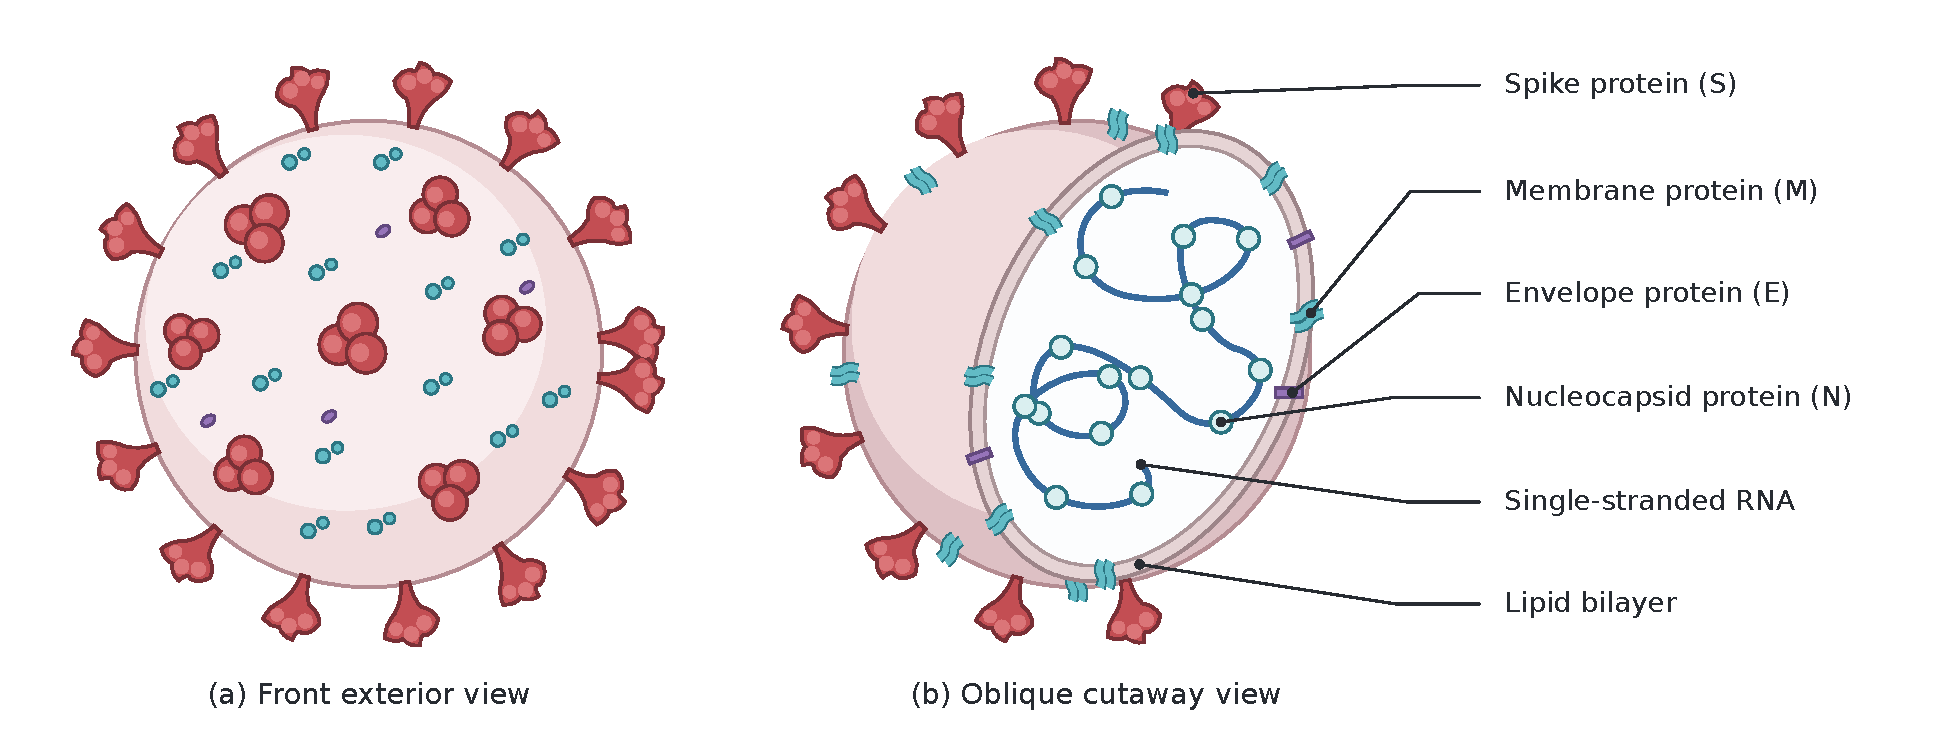
\includegraphics[width=0.52\columnwidth,trim=5bp 0bp 580bp 0bp,clip]{figures/sars-cov-2-structure-2d.pdf}\\[4pt]
    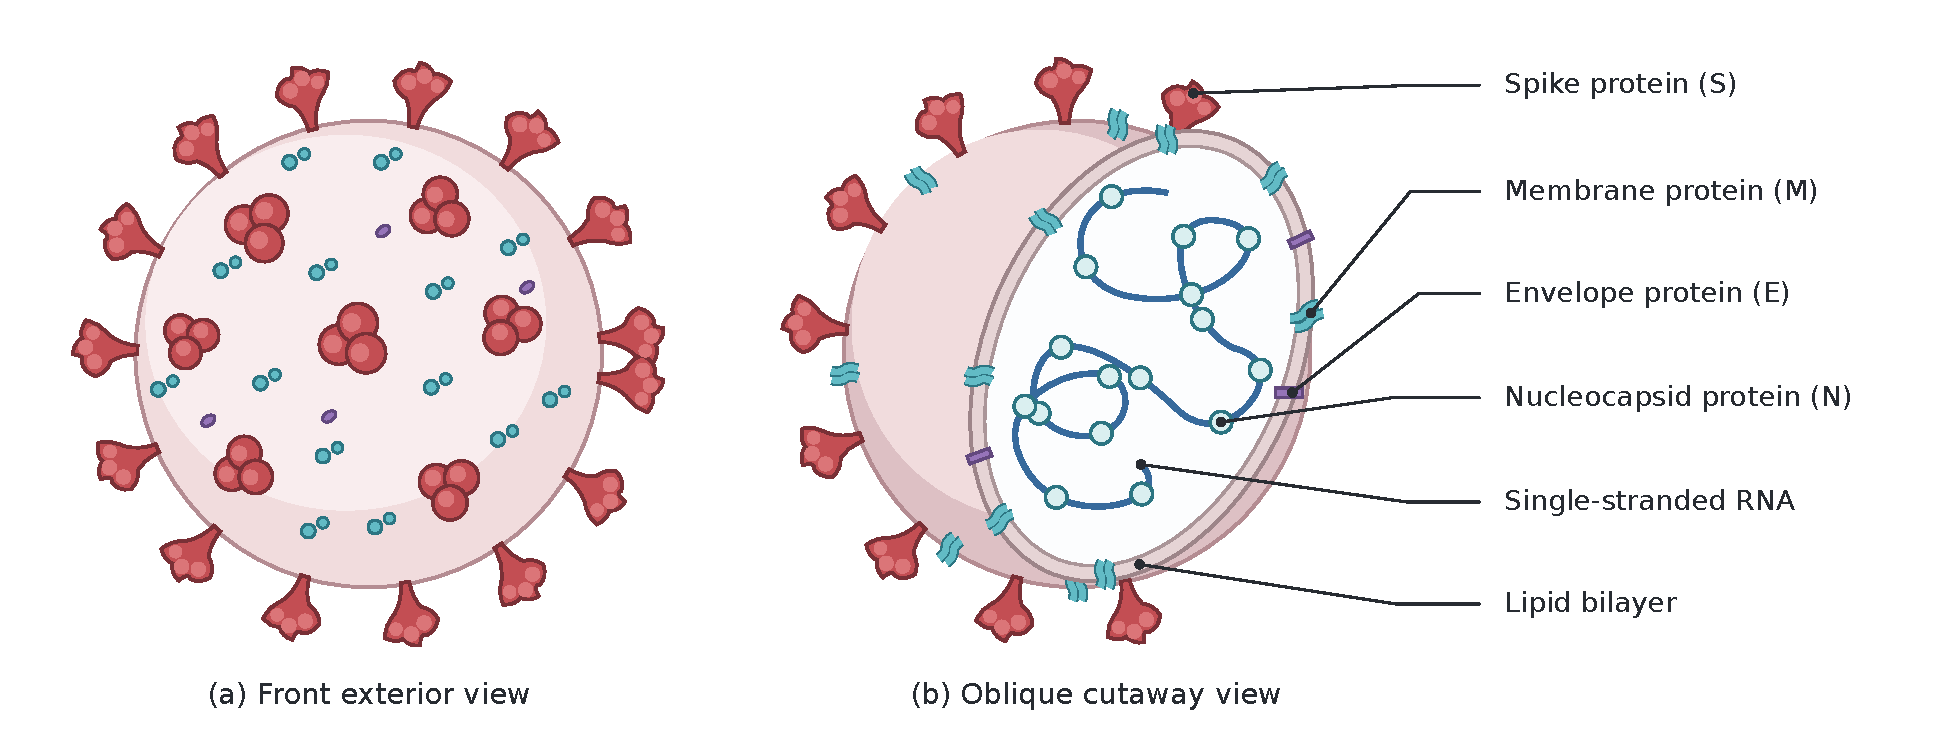
\includegraphics[width=\columnwidth,trim=365bp 0bp 0bp 0bp,clip]{figures/sars-cov-2-structure-2d.pdf}
    \caption{Schematic structure of SARS-CoV-2: (a) front exterior view; (b) oblique cutaway exposing the lipid bilayer and N-associated RNA. Leader lines identify the principal components. Original illustration following the NCBI structural overview~\cite{ncbiSarsStructure}; protein shapes, numbers, and dimensions are schematic and not to scale.}
    \label{fig:sars-structure}
\end{figure}

The viral genome is approximately 30~kb long, and its spike (S) region, located at roughly 21--25~kb, encodes the protein used to attach to host-cell membranes. This region also accumulates advantageous mutations, making spike sequences a useful source of information for studying viral lineages and sequence variation. The genome organization and the location of the S gene are shown in Fig.~\ref{fig:sars-genome}.

\begin{figure}[tbp]
    \centering
    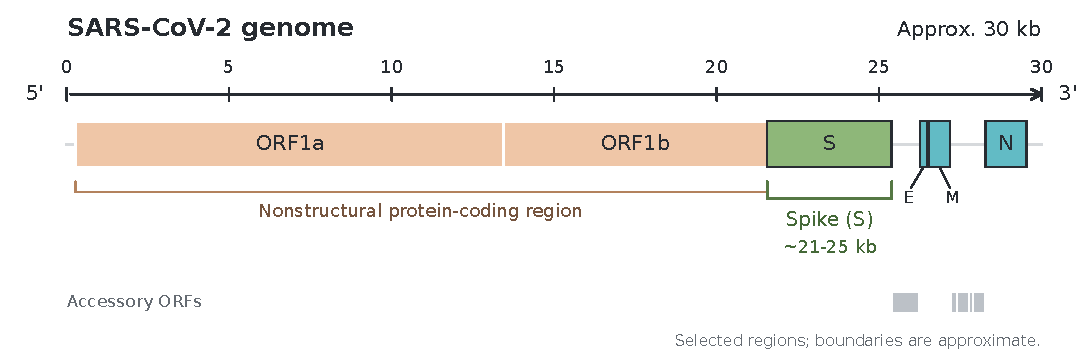
\includegraphics[width=\columnwidth]{figures/sars-cov-2-genome.pdf}
    \caption{Schematic of the approximately 30-kb SARS-CoV-2 genome, showing ORF1a and ORF1b, the structural protein-coding regions S, E, M, and N, and selected accessory ORFs. The S region at approximately 21--25~kb is highlighted. Genome overview follows Murad \textit{et al.}~\cite{murad2024snn}; boundaries are approximate, and the map does not depict individual amino-acid or nucleotide sequences.}
    \label{fig:sars-genome}
\end{figure}

% TODO (修正建議): add a Pango lineage tree figure here, with source and license.
Lineages are named by the dynamic Pango nomenclature~\cite{rambaut2020pango}. In practice, a lineage is assigned to a whole genome by phylogenetic placement or by models trained on aligned genomes: the pangolin tool~\cite{otoole2021pangolin} places genomes on a reference tree with UShER~\cite{turakhia2021usher}, and Nextclade~\cite{aksamentov2021nextclade} aligns them to a reference and assigns clades from their mutations. These tools rely on whole-genome alignment and curated trees. Machine-learning studies have therefore asked whether the spike sequence alone suffices. Murad \textit{et al.} classify spike sequences with an alignment-free pipeline based on spiking neural networks (SNNs)~\cite{murad2024snn}, and other pipelines turn sequences into signals or images for convolutional networks. These results show that spike sequences carry enough information to separate many lineages.

Biological sequences pose several challenges for such models. Protein sequences can have different lengths, while many conventional classifiers require fixed-size numerical inputs, so existing pipelines encode or transform sequences before classification. Murad \textit{et al.} use one-hot encoding with zero padding before an SNN classifier~\cite{murad2024snn}; SNNs represent information with temporally precise spikes and have been proposed as biologically inspired alternatives to conventional neural networks~\cite{maass1997,pfeiffer2018}. Signal- and image-based approaches add further transformations. On such tasks, strong classical baselines are already competitive.

Why consider a quantum model for this problem at all? The residual errors of strong classical models are not spread over all 22 lineages. They concentrate in a few groups of closely related lineages, the Delta sublineages and the early B.1 family, which are also the hardest lineages for every CNN baseline (Section~\ref{sec:res-baselines}). These lineages differ by few mutations, are not linearly separable in mutation space, and overlap even in a discriminant projection (Fig.~\ref{fig:lda-scatter}). Each group is thus a small nonlinear subproblem, with a few classes and a few thousand sequences, that calls for a nonlinear similarity measure, i.e., a kernel. Quantum kernels are a natural candidate for such subproblems: a quantum feature map embeds a few input coordinates into an exponentially large Hilbert space, and an entangling evolution makes every readout depend jointly on several coordinates through correlations that product-state encodings cannot generate~\cite{havlicek2019,huang2021power}. Whether this extra expressiveness helps on real biological data is an open question. There is no a priori reason to expect quantum structure in viral sequences, and quantum machine learning (QML) claims on such data rarely receive a controlled test against matched classical alternatives~\cite{bowles2024better}.

Among quantum models, we choose the projected quantum kernel (PQK)~\cite{huang2021power} for four reasons. (i) \emph{Attributability.} Variational quantum algorithms~\cite{cerezo2021vqa} must train their circuits and face optimization difficulties such as barren plateaus~\cite{mcclean2018barren}, so their performance differences are hard to attribute to the quantum features themselves. A PQK uses a fixed circuit with no trainable parameters as a feature map, reads out only single-qubit reduced density matrices, and passes them to a classical kernel machine, so any difference can only come from the feature map. (ii) \emph{Scalability.} Fidelity kernels~\cite{havlicek2019} concentrate exponentially in the number of qubits~\cite{thanasilp2024concentration}; a PQK compares only local reduced density matrices to mitigate this, and Huang \textit{et al.} show that it can outperform classical kernels on data with quantum structure. (iii) \emph{Cost.} A fidelity-kernel Gram matrix needs $O(N^2)$ circuits, about $4.5\times10^7$ for our largest group, whereas a PQK needs three measurement settings per sequence, $O(N)$ in total; it is the only quantum kernel that is practical at the size of our groups. (iv) \emph{Hardware fit.} It needs few qubits, native gates, and nearest-neighbor connectivity, so it can be simulated exactly today and run unchanged on near-term hardware. These properties make the PQK the quantum kernel whose contribution can be measured most cleanly on this task; this paper performs that measurement.

This paper asks one question: \emph{on spike-lineage classification, does a fixed quantum feature map add discriminative information beyond classical alternatives with the same interface?} To answer it, we make the following contributions:
\begin{enumerate}
    \item \textit{An attributable architecture.} QuSpike-PQK adds group-wise PQK experts as residual corrections to a strong linear reference; the quantum path has no trainable parameters, and a mixing weight of zero recovers the reference exactly (Section~\ref{sec:method}).
    \item \textit{A matched-control protocol.} Every quantum component is paired with a classical counterpart (identity kernel, random-Fourier-feature surrogate, entanglement-free circuit, width-matched MLP, ungrouped expert), and the decision criteria and stopping rule are fixed before evaluation (Section~\ref{sec:setup}).
    \item \textit{An empirical answer.} On 22 Pango lineages, QuSpike-PQK exceeds all one-hot and image-CNN baselines, but every quantum-specific comparison lies within noise: the PQK is classically replaceable, and the lead comes from the mutation-indicator representation (Section~\ref{sec:result}).
    \item \textit{A resource analysis.} We quantify the costs of PQK relative to fidelity kernels and to classical simulation, and derive necessary conditions for a resource crossover (Section~\ref{sec:theory}).
\end{enumerate}
Section~\ref{sec:related-work} reviews related work, Section~\ref{sec:discussion} discusses why the quantum features do not help here and when they could, and Section~\ref{sec:conclusion} concludes.

\section{Related Work}
\label{sec:related-work}

\textit{Spike-sequence classification.} Murad \textit{et al.}~\cite{murad2024snn} study alignment-free spike-sequence classification with an SNN; Maass~\cite{maass1997} and Pfeiffer and Pfeil~\cite{pfeiffer2018} describe the computational principles of spiking neural networks. Lineage assignment in genomic surveillance relies on whole-genome tools~\cite{rambaut2020pango,otoole2021pangolin,turakhia2021usher,aksamentov2021nextclade}.

\textit{Quantum kernel methods.} Havl\'{i}\v{c}ek \textit{et al.}~\cite{havlicek2019} build a fidelity kernel from a quantum feature space. Huang \textit{et al.}~\cite{huang2021power} propose the projected quantum kernel, which reads out only local reduced density matrices to mitigate the value concentration of fidelity kernels, and Thanasilp \textit{et al.}~\cite{thanasilp2024concentration} analyze the exponential concentration of quantum kernels. Variational quantum algorithms are reviewed by Cerezo \textit{et al.}~\cite{cerezo2021vqa}; their trainable circuits face barren plateaus~\cite{mcclean2018barren}.

\textit{Dequantization and benchmarking.} Schuld \textit{et al.}~\cite{schuld2021effect} show that data encoding determines a model's frequency spectrum. Schreiber \textit{et al.}~\cite{schreiber2023surrogates} and Sweke \textit{et al.}~\cite{sweke2023rff} show that band-limited quantum models can be approximated by classical surrogates such as random Fourier features. Bowles \textit{et al.}~\cite{bowles2024better} stress that quantum machine learning must be compared fairly against strong classical baselines. Our controls instantiate these surrogates and baselines directly.

\section{Method}
\label{sec:method}
% Method transcribed from Doc/QuSpike-PQK-方法論.md and verified against
% Research/QuSpike_PQK/{features,router,pqk,kernels,experts,pipeline,criteria}.py.

QuSpike-PQK is a \emph{classical--quantum hybrid} architecture: mutation encoding, the linear reference, routing, LDA, and the kernel-SVM experts all run on a classical computer, and only the Hamiltonian evolution that maps the reduced inputs to quantum features runs on a quantum circuit (here, a simulator). In one sentence: \emph{a strong, simple classical classifier answers first, and a quantum-kernel expert corrects it only on the most confusable lineages.} Four design principles fix the shape of the architecture:
\begin{enumerate}
    \item[P1)] \textit{No trainable quantum parameters.} The circuit depends only on the input and on the hyperparameters $(n,T,\tau,\gamma)$, which removes circuit optimization as an explanation for any outcome.
    \item[P2)] \textit{The strong classical baseline is a structural floor.} The quantum path enters as an additive correction whose weight can be zero.
    \item[P3)] \textit{Every quantum component has a classical counterpart} with an identical interface, so that its contribution can be isolated (Section~\ref{sec:controls}).
    \item[P4)] \textit{Decision criteria and a stopping rule are fixed before evaluation} (Section~\ref{sec:criteria}).
\end{enumerate}

% TODO: verify that Huang et al. (2021) use a Trotterized 1D Heisenberg
% evolution as their Hamiltonian-evolution feature map.
\textit{Why these components.} Each component answers a specific constraint of the problem. \emph{Residual, group-wise experts:} the linear reference already separates most lineages (group O, Fig.~\ref{fig:lda-scatter}), so a nonlinear model is needed only on the few groups where it fails, and adding it as a correction keeps the reference as a floor (P2). \emph{A kernel machine:} each group is a small problem (4--7 classes, $10^3$--$10^4$ sequences) for which a kernel SVM is convex, data-efficient, and needs no circuit training (P1). \emph{A projected quantum kernel:} it supplies the nonlinear similarity with a fixed circuit, needs $O(N)$ rather than $O(N^2)$ circuits (Section~\ref{sec:resources}), and mitigates the concentration of fidelity kernels~\cite{huang2021power}. \emph{A Trotterized Heisenberg evolution:} Hamiltonian-evolution feature maps are the family used for projected quantum kernels by Huang \textit{et al.}~\cite{huang2021power}; Heisenberg couplings decompose into native two-qubit rotations, their SU(2) symmetry makes the map analyzable (Propositions~1 and~2), and switching them off yields a closed-form classical kernel that serves directly as the entanglement control C3 (P3). \emph{An LDA projection:} a few qubits accept only a few inputs, so the 3,686-dimensional input is first reduced to the directions that discriminate within the group.

\subsection{Problem Formulation and Notation}
\label{sec:formulation}

Let $\mathcal{D}_{\mathrm{tr}}=\{(s_i,y_i)\}_{i=1}^{N}$ be the training set of spike sequences $s_i$ with lineage labels $y_i\in\mathcal{Y}=\{1,\dots,C\}$, $C=22$, and let $M$ denote the number of test sequences. The label set is partitioned into three groups by a fixed map $\pi:\mathcal{Y}\to\mathcal{G}=\{\mathrm{D},\mathrm{B},\mathrm{O}\}$:
\begin{itemize}
    \item $\mathcal{Y}_{\mathrm{D}}$ (Delta): B.1.617.2, AY.103, AY.2, AY.25, AY.3, AY.4, and AY.44 ($C_{\mathrm{D}}=7$);
    \item $\mathcal{Y}_{\mathrm{B}}$ (B.1 family): B.1, B.1.1, B.1.2, and B.1.177 ($C_{\mathrm{B}}=4$);
    \item $\mathcal{Y}_{\mathrm{O}}$: the remaining 11 lineages.
\end{itemize}
% TODO: state that the earlier-stage error analysis used training/validation
% data only (not the test split).
The two groups $\mathcal{Q}=\{\mathrm{D},\mathrm{B}\}$ consist of closely related lineages on which a linear reference classifier concentrated its errors in an earlier stage of this study; only these groups receive a quantum expert. Their lineages also overlap in the discriminant projection (Fig.~\ref{fig:lda-scatter}, Section~\ref{sec:projection}). Group $g\in\mathcal{Q}$ uses $n_g$ qubits, with $n_{\mathrm{D}}=4$ and $n_{\mathrm{B}}=2$; $N_g$ denotes the number of training sequences whose label lies in $\mathcal{Y}_g$.

\subsection{Overall Architecture}
\label{sec:architecture}

Figure~\ref{fig:pqk-architecture} summarizes the model. A sequence is encoded as a binary mutation vector $x$, scored by a linear reference classifier, and routed by the reference prediction. Sequences routed to $\mathcal{Q}$ are projected to a low-dimensional discriminant space, mapped through the quantum feature map, and scored by a group-specific kernel expert whose output is added to the reference logits:
\begin{equation}
    \ell(x)=\ell_{\mathrm{ref}}(x)
    +s\sum_{g\in\mathcal{Q}}\mathbb{1}[r(x)=g]\,P_g\,f_g\!\big(\phi_g(z_g(x))\big).
    \label{eq:master}
\end{equation}
Here $\ell_{\mathrm{ref}}$ is the reference logit vector (Section~\ref{sec:router}), $r$ the router, $z_g$ the group projection (Section~\ref{sec:projection}), $\phi_g$ the quantum feature map (Section~\ref{sec:encoding}), $f_g$ the kernel expert (Section~\ref{sec:kernel}), $P_g\in\{0,1\}^{C\times C_g}$ the embedding of group scores into the $C$ logits, and $s\ge 0$ a mixing weight selected on validation data (Section~\ref{sec:fusion}).

\begin{figure}[!t]
    \centering
    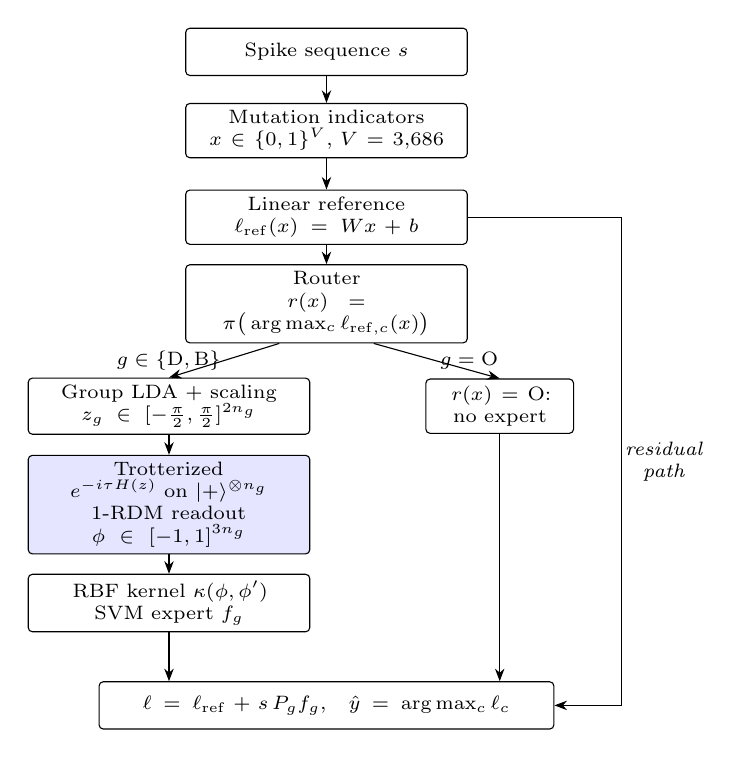
\begin{tikzpicture}[
        box/.style={draw, rounded corners=1.5pt, align=center, font=\scriptsize,
                    inner sep=2.5pt, minimum height=6mm, text width=3.4cm},
        qbox/.style={box, fill=blue!10},
        arr/.style={-{Stealth[length=1.6mm]}, thin},
        lab/.style={font=\scriptsize\itshape, inner sep=1pt}]
        \node[box] (seq) at (0,0) {Spike sequence $s$};
        \node[box] (mut) at (0,-1.0) {Mutation indicators\\ $x\in\{0,1\}^{V}$, $V=3{,}686$};
        \node[box] (ref) at (0,-2.1) {Linear reference\\ $\ell_{\mathrm{ref}}(x)=Wx+b$};
        \node[box] (route) at (0,-3.2) {Router\\ $r(x)=\pi\big(\arg\max_c \ell_{\mathrm{ref},c}(x)\big)$};
        \node[box] (lda) at (-2.0,-4.5) {Group LDA + scaling\\ $z_g\in[-\tfrac{\pi}{2},\tfrac{\pi}{2}]^{2n_g}$};
        \node[qbox] (pqk) at (-2.0,-5.75) {Trotterized $e^{-i\tau H(z)}$ on $|{+}\rangle^{\otimes n_g}$\\ 1-RDM readout $\phi\in[-1,1]^{3n_g}$};
        \node[box] (svm) at (-2.0,-7.0) {RBF kernel $\kappa(\phi,\phi')$\\ SVM expert $f_g$};
        \node[box, text width=1.7cm] (easy) at (2.2,-4.5) {$r(x)=\mathrm{O}$:\\ no expert};
        \node[box, text width=5.6cm] (fuse) at (0,-8.3) {$\ell=\ell_{\mathrm{ref}}+s\,P_g f_g$,\quad $\hat{y}=\arg\max_c \ell_c$};
        \draw[arr] (seq) -- (mut);
        \draw[arr] (mut) -- (ref);
        \draw[arr] (ref) -- (route);
        \draw[arr] (route.south) ++(-0.6,0) -- node[lab, left] {$g\in\{\mathrm{D},\mathrm{B}\}$} (lda.north);
        \draw[arr] (route.south) ++(0.6,0) -- node[lab, right] {$g=\mathrm{O}$} (easy.north);
        \draw[arr] (lda) -- (pqk);
        \draw[arr] (pqk) -- (svm);
        \draw[arr] (svm.south) -- (svm.south |- fuse.north);
        \draw[arr] (easy.south) -- (easy.south |- fuse.north);
        \draw[arr] (ref.east) -- (3.75,-2.1) -- node[lab, right, align=center] {residual\\ path} (3.75,-8.3) -- (fuse.east);
    \end{tikzpicture}
    \caption{QuSpike-PQK architecture. The linear reference both supplies the residual logits and routes each sequence. Only sequences routed to the Delta (D) or B.1-family (B) groups pass through the quantum feature map (shaded); the quantum path has no trainable parameters, and $s=0$ recovers the reference exactly.}
    \label{fig:pqk-architecture}
\end{figure}

\subsection{Mutation-Indicator Representation}
\label{sec:mutations}

Mutation encoding has two steps: each sequence is aligned to the reference and its mutations are listed, and the mutations are then encoded as a fixed-length 0/1 vector.

\textbf{Step 1: sequence $\to$ mutation set.} The reference is the Wuhan-Hu-1 spike protein $R$ (NCBI YP\_009724390.1, $|R|=1{,}273$ residues). Sequences of the same length as $R$ are compared position by position; sequences of different length are aligned with Python's \texttt{difflib.SequenceMatcher}. Each difference is recorded as a token $(p,a)$ with 1-based reference position $p$:
\begin{itemize}
    \item \emph{Substitutions} are recorded as (position, new amino acid), e.g., D614G as (614, G);
    \item \emph{internal deletions} as (position, ``-''), e.g., the 156--157 deletion of Delta;
    \item \emph{terminal truncations} are treated as unobserved, not as deletions; \emph{insertions} are ignored;
    \item positions with the unknown symbol \texttt{X} are discarded.
\end{itemize}

\textbf{Step 2: mutation set $\to$ 0/1 vector.} The vocabulary $\mathcal{V}$ is built from training sequences only: all distinct (position, amino acid) tokens, sorted, giving $V=|\mathcal{V}|=3{,}686$. For each sequence, the entries of the mutations it carries are set to 1 and all others to 0,
\begin{equation}
    x_v(s)=\mathbb{1}[v\in m(s)],\qquad v\in\mathcal{V},
    \label{eq:mutation}
\end{equation}
where $m(s)$ is the mutation set from Step 1. Test-set mutations absent from the training vocabulary are dropped rather than added as dimensions, so that no test information leaks into the features. For example, a Delta sequence with mutations at L452R, T478K, and D614G has ones at those entries and zeros elsewhere. The 22,175 training sequences form a $22{,}175\times3{,}686$ matrix, which is the input of both the linear reference and the LDA.
% TODO: state on which split the ESM-2 comparison was made, and its score.
We also evaluated frozen protein language-model embeddings (ESM-2, 150M parameters, mean-pooled), to be adopted only if they exceeded the mutation-indicator reference by more than 0.02 in macro-F1; they scored lower, so $x$ is used throughout, and all controls share it.

\subsection{Linear Reference and Classical Router}
\label{sec:router}

The reference classifier is a linear softmax model,
\begin{equation}
    \ell_{\mathrm{ref}}(x)=Wx+b,\qquad W\in\mathbb{R}^{C\times V},\ b\in\mathbb{R}^{C},
    \label{eq:reference}
\end{equation}
trained with cross-entropy and AdamW (learning rate $3\times10^{-3}$, weight decay $10^{-4}$, batch size 512, 60 epochs). It plays three roles: control C0, the structural floor of \eqref{eq:master}, and the router
\begin{equation}
    r(x)=\pi\big(\hat{c}_{\mathrm{ref}}(x)\big),\qquad \hat{c}_{\mathrm{ref}}(x)=\arg\max_{c}\ell_{\mathrm{ref},c}(x).
    \label{eq:router}
\end{equation}
A sequence routed to the wrong group cannot be helped by the correct expert. We report the routing accuracy
\begin{equation}
    \rho=\frac{1}{M}\sum_{j=1}^{M}\mathbb{1}\big[r(x_j)=\pi(y_j)\big],
    \label{eq:routing-accuracy}
\end{equation}
the share of test sequences routed to their true group, and, for $g\in\mathcal{Q}$, the group recall
\begin{equation}
    \rho_g=\frac{\sum_{j}\mathbb{1}\big[\pi(y_j)=g,\ r(x_j)=g\big]}{\sum_{j}\mathbb{1}\big[\pi(y_j)=g\big]},
    \label{eq:routing-recall}
\end{equation}
which upper-bounds the share of group-$g$ test sequences that reach their own expert.

\subsection{Group-Wise Discriminant Projection}
\label{sec:projection}

The circuit of group $g$ accepts at most $2n_g$ real inputs ($n_g$ single-qubit fields and up to $n_g$ couplings), whereas $V=3{,}686$. For each $g\in\mathcal{Q}$, linear discriminant analysis (LDA)~\cite{fisher1936} is fitted on the training sequences of $\mathcal{Y}_g$ only. Let $A_g\in\mathbb{R}^{V\times k_g}$ collect the leading solutions of $S_{b}a=\lambda S_{w}a$, where $S_b$ and $S_w$ are the between- and within-class scatter matrices, with
\begin{equation}
    k_g=\min(C_g-1,\,2n_g),\qquad k_{\mathrm{D}}=6,\quad k_{\mathrm{B}}=3.
\end{equation}
With $u=A_g^{\top}x$ and per-coordinate training quantiles $q^{\mathrm{lo}}_j$ (1st percentile) and $q^{\mathrm{hi}}_j$ (99th percentile),
\begin{equation}
    z_j=\pi\,\frac{\operatorname{clip}(u_j;\,q^{\mathrm{lo}}_j,q^{\mathrm{hi}}_j)-q^{\mathrm{lo}}_j}{q^{\mathrm{hi}}_j-q^{\mathrm{lo}}_j}-\frac{\pi}{2},\qquad j\le k_g,
    \label{eq:scaling}
\end{equation}
and $z_j=0$ for $k_g<j\le 2n_g$ (zero padding; Fig.~\ref{fig:projection}). LDA is preferred over PCA because, within an already selected group, the directions of largest variance are generally not the discriminative ones. Quantile clipping prevents outliers from compressing the dynamic range. The interval $[-\pi/2,\pi/2]$ keeps the total field rotation $2\tau z_j$ within $[-0.8\pi,0.8\pi]$ for $\tau=0.8$, so that distinct inputs give distinct rotations (Proposition~2 below).

Figure~\ref{fig:lda-scatter} shows the resulting projections. The ratio of mean centroid distance to within-class standard deviation is 2.60 for D and 2.43 for B, against 12.9 for group O (projected the same way for comparison only). The two expert groups are thus the poorly separated ones, which is consistent with giving group O no expert.

\begin{figure*}[!t]
    \centering
    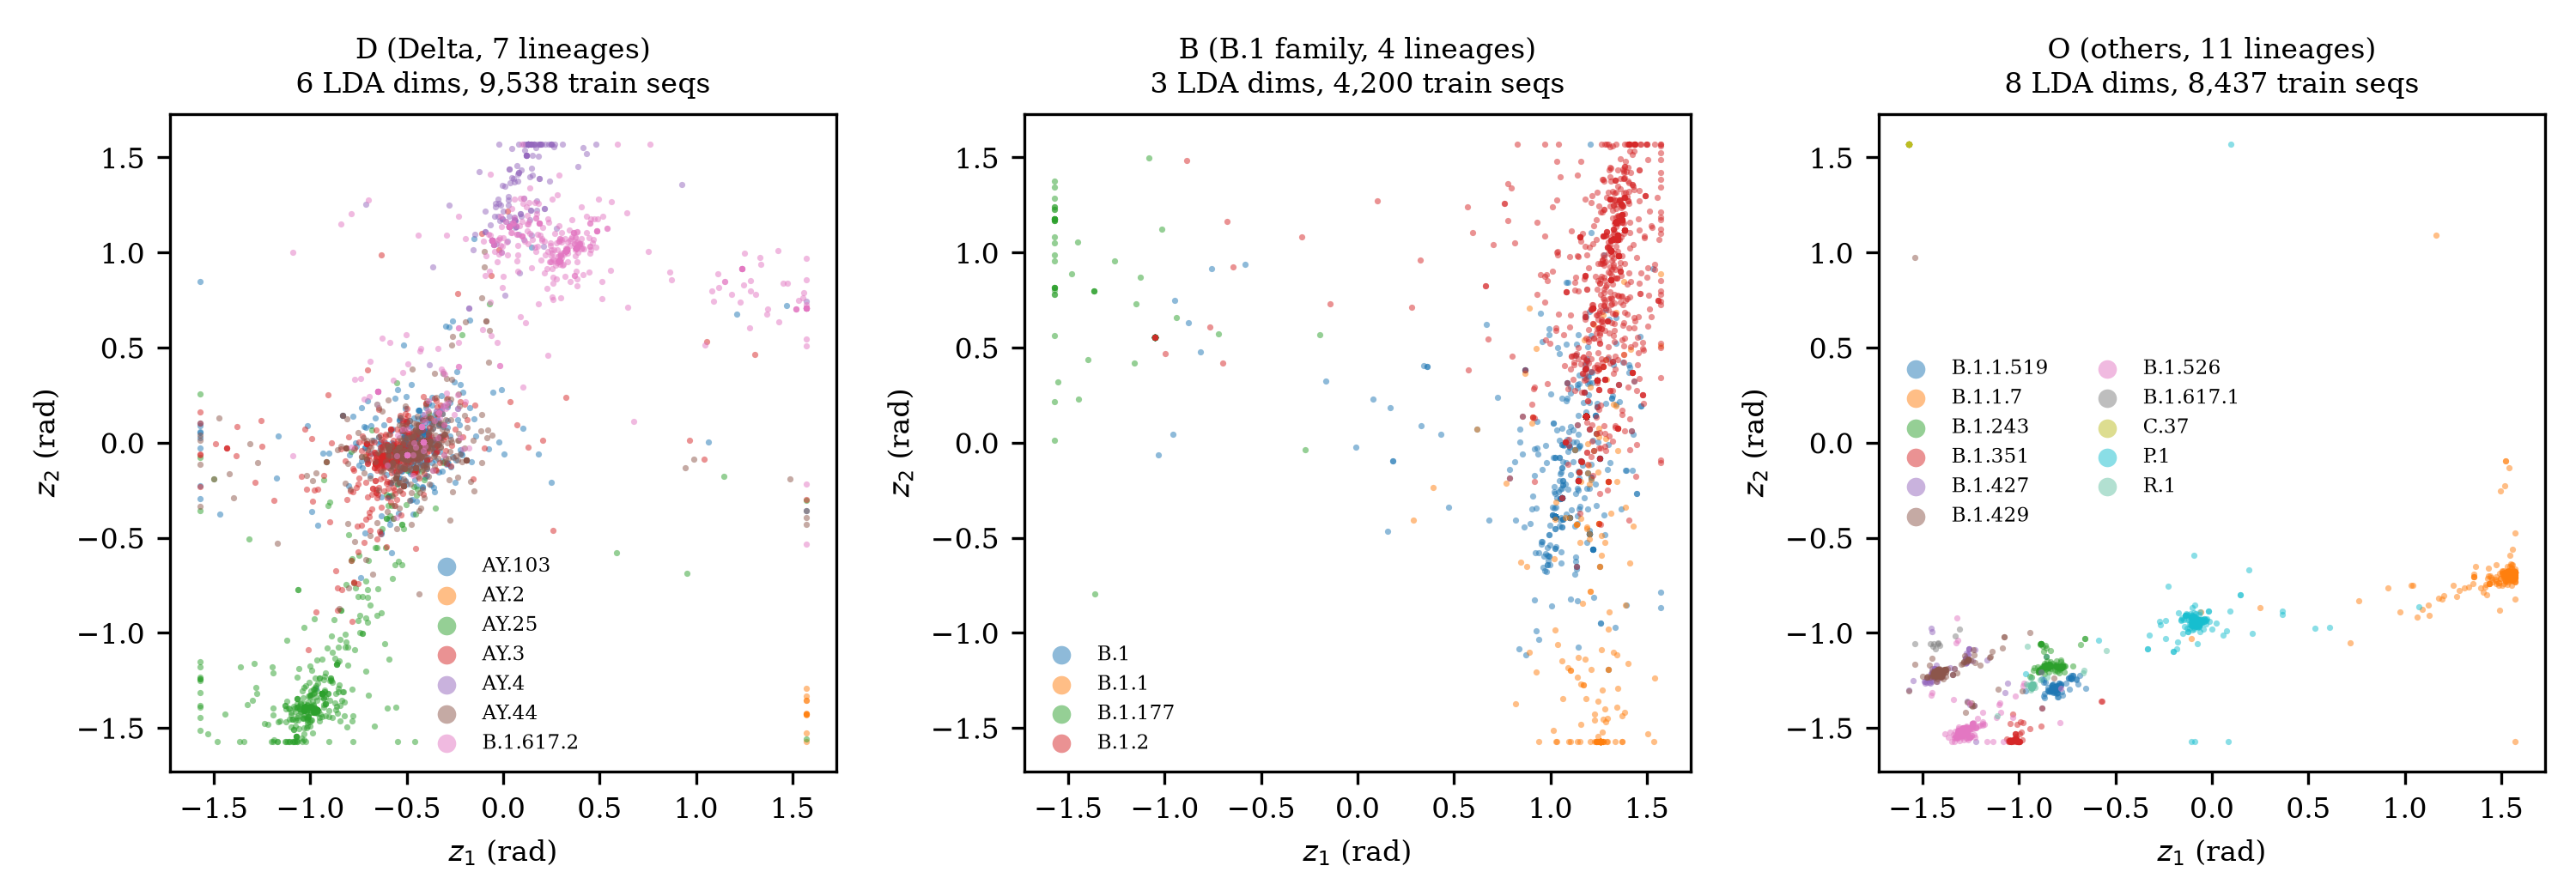
\includegraphics[width=0.78\textwidth]{figures/z1z2.png}
    \caption{LDA projections of the training sequences of groups D, B, and O (left to right; first two axes $z_1$, $z_2$ after scaling, in rad; 3,000 points each, colored by lineage; LDA fitted on the training set only). D: AY.25, AY.4, and B.1.617.2 separate, while AY.103, AY.3, and AY.44 overlap; B: B.1.177 is isolated, while B.1, B.1.1, and B.1.2 spread along one band; O: compact, well-separated clusters (group O does not enter the quantum path; shown for comparison only). The mean centroid distance over within-class standard deviation is 2.60, 2.43, and 12.91 for D, B, and O, and the shares of sequences clipped at $\pm\pi/2$ are 10.0\%, 7.1\%, and 11.9\%.}
    \label{fig:lda-scatter}
\end{figure*}

\begin{figure}[!t]
    \centering
    \resizebox{\columnwidth}{!}{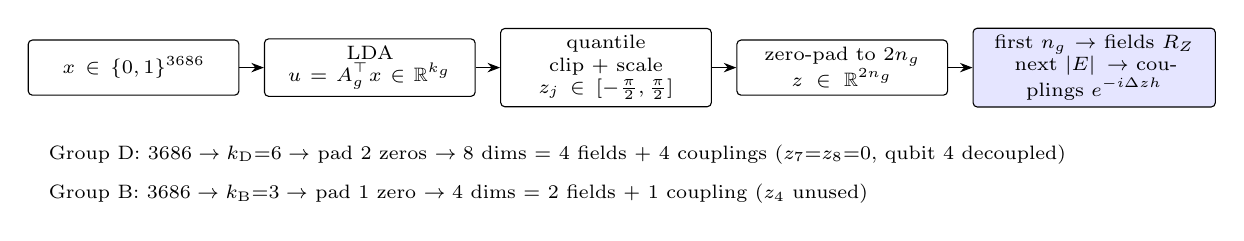
\begin{tikzpicture}[
        box/.style={draw, rounded corners=1.5pt, align=center, font=\scriptsize, inner sep=2.5pt, minimum height=7mm, text width=2.5cm},
        qbox/.style={box, fill=blue!10},
        arr/.style={-{Stealth[length=1.6mm]}, thin}]
        \node[box] (x) at (0,0) {$x\in\{0,1\}^{3686}$};
        \node[box] (lda) at (3.0,0) {LDA\\ $u=A_g^{\top}x\in\mathbb{R}^{k_g}$};
        \node[box] (sc) at (6.0,0) {quantile clip + scale\\ $z_j\in[-\tfrac{\pi}{2},\tfrac{\pi}{2}]$};
        \node[box] (pad) at (9.0,0) {zero-pad to $2n_g$\\ $z\in\mathbb{R}^{2n_g}$};
        \node[qbox, text width=2.9cm] (q) at (12.2,0) {first $n_g\to$ fields $R_Z$\\ next $|E|\to$ couplings $e^{-i\Delta z h}$};
        \draw[arr] (x)--(lda); \draw[arr] (lda)--(sc); \draw[arr] (sc)--(pad); \draw[arr] (pad)--(q);
        \node[font=\scriptsize, anchor=west, align=left] at (-1.2,-1.1) {Group D: $3686\to k_{\mathrm{D}}{=}6\to$ pad 2 zeros $\to8$ dims $=$ 4 fields $+$ 4 couplings ($z_7{=}z_8{=}0$, qubit 4 decoupled)};
        \node[font=\scriptsize, anchor=west, align=left] at (-1.2,-1.6) {Group B: $3686\to k_{\mathrm{B}}{=}3\to$ pad 1 zero $\to4$ dims $=$ 2 fields $+$ 1 coupling ($z_4$ unused)};
    \end{tikzpicture}}
    \caption{Group-wise discriminant projection: LDA fitted on the group's training sequences gives $k_g$ discriminant directions, which are quantile-clipped and scaled into circuit angles; dimensions short of $2n_g$ are zero-padded. The first $n_g$ act as local fields and the next $|E|$ as nearest-neighbor couplings.}
    \label{fig:projection}
\end{figure}

\subsection{Hamiltonian-Evolution Encoding}
\label{sec:encoding}

For $n=n_g$ qubits and input $z\in[-\pi/2,\pi/2]^{2n}$, define the Heisenberg-type Hamiltonian
\begin{equation}
    H(z)=\sum_{j=1}^{n}z_jZ_j+\sum_{e=(j,j')\in E}z_{n+j}\,h_{jj'},
    \label{eq:hamiltonian}
\end{equation}
\begin{equation}
    h_{jj'}=X_jX_{j'}+Y_jY_{j'}+Z_jZ_{j'},
\end{equation}
where $E=\{(j,\,j\bmod n+1)\}_{j=1}^{n}$ is the ring for $n\ge3$ ($|E|=n$) and $E=\{(1,2)\}$ for $n=2$ ($|E|=1$, input $z_4$ unused). The first $n$ inputs act as local fields and the next $|E|$ as nearest-neighbor couplings. With $\Delta=\tau/T$, the first-order Trotterized evolution is
\begin{equation}
    U_T(z)=\prod_{t=1}^{T}\Bigg[\prod_{(j,j')\in E}e^{-i\Delta z_{n+j}h_{jj'}}\prod_{j=1}^{n}e^{-i\Delta z_jZ_j}\Bigg],
    \label{eq:trotter}
\end{equation}
applied to $|\psi_0\rangle=|{+}\rangle^{\otimes n}=H_{\mathrm{d}}^{\otimes n}|0\rangle^{\otimes n}$, where $H_{\mathrm{d}}$ is the Hadamard gate. We use $T=4$ and $\tau=0.8$. Every factor is native to gate-model hardware: $e^{-i\Delta z Z}=R_Z(2\Delta z)$, and because $XX$, $YY$, and $ZZ$ commute pairwise,
\begin{equation}
    e^{-i\Delta J h_{jj'}}=R_{XX}(2\Delta J)\,R_{YY}(2\Delta J)\,R_{ZZ}(2\Delta J)
\end{equation}
holds exactly. Moreover, $h_{jj'}=2\,\mathrm{SWAP}_{jj'}-I$, so each coupling is a partial swap,
\begin{equation}
    e^{-i\alpha h_{jj'}}=e^{i\alpha}\big[\cos(2\alpha)\,I-i\sin(2\alpha)\,\mathrm{SWAP}_{jj'}\big].
    \label{eq:partial-swap}
\end{equation}
Entanglement therefore arises from the interplay between partial swaps and inhomogeneous fields $z_j\neq z_{j'}$.

The classifier is defined by the circuit $U_T$ itself, so Trotter error is not an approximation error of the model; it only measures how closely the feature map follows the continuous dynamics $e^{-i\tau H(z)}$. The first-order bound~\cite{lloyd1996,childs2021trotter}
\begin{equation}
    \big\|U_T(z)-e^{-i\tau H(z)}\big\|\le\frac{\tau^2}{2T}\sum_{a<b}\big\|[H_a,H_b]\big\|=O\!\left(\frac{n\tau^2}{T}\right)
    \label{eq:trotter-error}
\end{equation}
applies because each term $H_a$ has norm $O(1)$ for $|z_j|\le\pi/2$ and fails to commute with only $O(1)$ neighboring terms.
% TODO: report the same diagnostic at the operating point (n = 2, 4; tau = 0.8).
Numerically ($n=3$, $\tau=0.7$; Fig.~\ref{fig:viz-encoding}c), the largest readout deviation $\max_i|\phi_i-\phi_{\mathrm{exact},i}|$, averaged over 40 random $z$, decreases from $1.93\times10^{-1}$ at $T=4$ to $3.05\times10^{-3}$ at $T=256$ (log-log slope $-0.997$), consistent with $O(1/T)$. At $T=4$ the feature map is thus a coarse discretization of the continuous dynamics, and the name ``Hamiltonian evolution'' describes its construction rather than a faithful simulation.

\textit{Projected readout.} With $|\psi(z)\rangle=U_T(z)|\psi_0\rangle$ and $\rho_k(z)=\operatorname{Tr}_{\neg k}|\psi(z)\rangle\langle\psi(z)|$ the one-qubit reduced density matrix (1-RDM), $\rho_k=\tfrac12(I+\phi_k\cdot\boldsymbol{\sigma})$ with Bloch vector
\begin{equation}
    \phi_k(z)=\big(\langle X_k\rangle,\langle Y_k\rangle,\langle Z_k\rangle\big)_{\psi(z)},
\end{equation}
\begin{equation}
    \phi(z)=\big(\phi_1(z),\dots,\phi_n(z)\big)\in[-1,1]^{3n}.
    \label{eq:readout}
\end{equation}
The feature vector is thus exactly the collection of 1-RDMs. Two structural properties of this map (Fig.~\ref{fig:viz-encoding} shows the circuit and numerical examples) follow directly from \eqref{eq:hamiltonian}--\eqref{eq:trotter}.

\textit{Proposition 1 (conserved magnetization).} For all $z$,
\[
    \sum_{k=1}^{n}\langle Z_k\rangle_{\psi(z)}=0.
\]

\textit{Proof.} The total magnetization $\sum_k Z_k$ commutes with every $Z_j$ and, by the SU(2) invariance of $h_{jj'}$, with every coupling gate; hence it is conserved by $U_T(z)$. Its expectation in $|{+}\rangle^{\otimes n}$ is zero. $\blacksquare$

Consequently, $\phi(z)$ lies in a hyperplane of dimension $3n-1$; for $n=2$, $\langle Z_1\rangle=-\langle Z_2\rangle$.

\textit{Proposition 2 (product-state limit).} If all couplings vanish, then for every $T$
\begin{equation}
    \phi_k(z)=\big(\cos 2\tau z_k,\ \sin 2\tau z_k,\ 0\big).
    \label{eq:product-limit}
\end{equation}

\textit{Proof.} The qubits evolve independently under $R_Z(2\tau z_k)$, whose action on $|{+}\rangle$ rotates the Bloch vector $(1,0,0)$ by angle $2\tau z_k$ about the $z$-axis. $\blacksquare$

The implementation agrees with \eqref{eq:product-limit} to $2.22\times10^{-15}$. Because $2\tau|z_k|\le0.8\pi<\pi$, this map is injective on $[-\pi/2,\pi/2]$. Proposition~2 also fixes a consequence of zero padding: in group D, $k_{\mathrm{D}}=6<8$ gives $z_7=z_8=0$, so the couplings on edges $(3,4)$ and $(4,1)$ vanish. Qubit 4 is then decoupled, its readout is given by \eqref{eq:product-limit}, and entangling dynamics are confined to the path $1$--$2$--$3$. In group B, $k_{\mathrm{B}}=3$ fills the two fields and the single coupling, so padding does not remove an edge.

\textit{Frequency content.} Following Schuld \textit{et al.}~\cite{schuld2021effect}, each entry of $\phi$ is a trigonometric polynomial of $z$. A field input enters through $T$ generators $\Delta Z$ with eigenvalue gap $2\Delta$, and a coupling input through $T$ generators $\Delta h$ whose eigenvalues $\{1,-3\}$ have gap $4\Delta$. The accessible frequencies are therefore $\{2\Delta m:|m|\le T\}$ (maximum $2\tau$) for fields and $\{4\Delta m:|m|\le T\}$ (maximum $4\tau$) for couplings. This band limit is what admits classical surrogates (Section~\ref{sec:controls}).

\begin{figure*}[!t]
    \centering
    \noindent\textbf{(a)}\hfill\null\\[-2pt]
    \resizebox{0.62\textwidth}{!}{%
    \begin{quantikz}[row sep=0.2cm, column sep=0.3cm, font=\small]
        \lstick{$q_1$} & \gate{H_{\mathrm{d}}} & \gate{R_Z(2\Delta z_1)}\gategroup[4,steps=3,style={dashed,rounded corners,inner xsep=3pt,inner ysep=4pt},label style={label position=below,anchor=north,yshift=-0.25cm}]{repeat $T$ times} & \gate[2]{e^{-i\Delta z_5 h}} & \qw & \gate[4]{e^{-i\Delta z_8 h}} & \meter{} & \rstick{$\phi_1$}\\
        \lstick{$q_2$} & \gate{H_{\mathrm{d}}} & \gate{R_Z(2\Delta z_2)} & & \gate[2]{e^{-i\Delta z_6 h}} & & \meter{} & \rstick{$\phi_2$}\\
        \lstick{$q_3$} & \gate{H_{\mathrm{d}}} & \gate{R_Z(2\Delta z_3)} & \gate[2]{e^{-i\Delta z_7 h}} & & & \meter{} & \rstick{$\phi_3$}\\
        \lstick{$q_4$} & \gate{H_{\mathrm{d}}} & \gate{R_Z(2\Delta z_4)} & & \qw & & \meter{} & \rstick{$\phi_4$}
    \end{quantikz}}\\[2pt]
    \begin{minipage}[t]{0.40\textwidth}\centering
        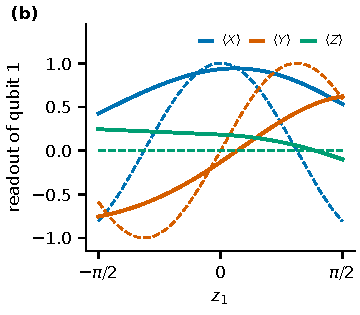
\includegraphics[width=\linewidth]{figures/fig_readout.pdf}
    \end{minipage}\hspace{0.04\textwidth}
    \begin{minipage}[t]{0.40\textwidth}\centering
        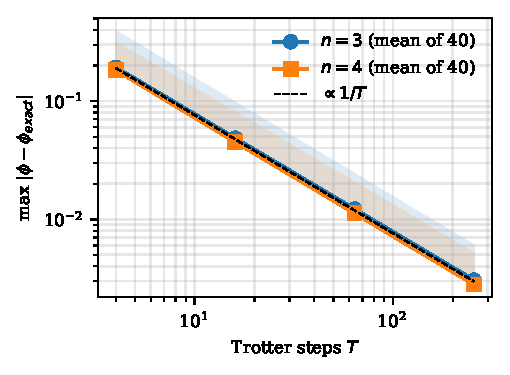
\includegraphics[width=\linewidth]{figures/trotter_error.pdf}
    \end{minipage}
    \caption{Visualization of the quantum feature map. (a) Circuit for group D ($n=4$): $H_{\mathrm{d}}$ prepares $|{+}\rangle^{\otimes4}$, $T$ Trotter steps are repeated ($R_Z$ fields and four ring couplings $e^{-i\Delta z h}$), and the Bloch vector $\phi_k$ of each qubit is read out. (b) Readout of qubit 1 while sweeping $z_1$ with the other inputs fixed ($n{=}4$, $T{=}4$, $\tau{=}0.8$): solid, MAIN; dashed, the coupling-free C3 ($\cos2\tau z,\ \sin2\tau z,\ 0$, Proposition~2); dotted, ridge regression with 24 random Fourier features on this one-dimensional slice (RMSE $\approx0.002$), showing that the band-limited map is RFF-approximable. (c) Trotter error versus $T$: largest readout deviation $\max_i|\phi_i-\phi_{\mathrm{exact},i}|$ from exact evolution ($\tau{=}0.7$; each point is the mean over 40 random $z$, shading is the min--max range); the log-log slope is about $-1$, consistent with $O(1/T)$.}
    \label{fig:viz-encoding}
\end{figure*}

\subsection{Projected Quantum Kernel and Group Experts}
\label{sec:kernel}

Huang \textit{et al.}~\cite{huang2021power} define the projected quantum kernel
\begin{equation}
    k^{\mathrm{PQ}}(z,z')=\exp\!\Big(-\gamma'\sum_{k=1}^{n}\big\|\rho_k(z)-\rho_k(z')\big\|_F^2\Big).
\end{equation}
Since $\|\rho_k-\rho_k'\|_F^2=\tfrac12\|\phi_k-\phi_k'\|_2^2$, this is the Gaussian kernel on the readout,
\begin{equation}
    \kappa(z,z')=\exp\!\big(-\gamma\,\|\phi(z)-\phi(z')\|_2^2\big),\qquad\gamma=\gamma'/2,
    \label{eq:pqk}
\end{equation}
which is positive definite by construction. The bandwidth follows the median heuristic,
\begin{equation}
    \gamma=\Big(2\operatorname*{median}_{a<b}\|\phi_a-\phi_b\|_2^2\Big)^{-1},
    \label{eq:median-gamma}
\end{equation}
estimated on 512 training samples of the group. Projection to local 1-RDMs, rather than the fidelity kernel $|\langle\psi(z)|\psi(z')\rangle|^2$~\cite{havlicek2019}, is the mechanism proposed in~\cite{huang2021power} to mitigate the kernel-value concentration of large Hilbert spaces.

For each $g\in\mathcal{Q}$, the expert $f_g$ is a multiclass support vector machine with precomputed Gram matrix $K_g=[\kappa(z_a,z_b)]\in\mathbb{R}^{N_g\times N_g}$ and regularization $C_{\mathrm{SVM}}=10$. It is trained one-vs-one: each of the $C_g(C_g-1)/2$ pairwise classifiers has the decision function
\begin{equation}
    f^{(c,c')}_g(x)=\sum_{a\in\mathrm{SV}_{cc'}}\beta^{(cc')}_{a}\,\kappa\big(z_g(x),z_a\big)+b_{cc'},
    \label{eq:svm}
\end{equation}
and the per-class scores $f_{g,c}$, $c\in\mathcal{Y}_g$, are the one-vs-rest aggregation of the pairwise votes and confidences (scikit-learn \texttt{decision\_function\_shape="ovr"}). Floating-point round-off can break positive semidefiniteness; if $\lambda_{\min}(K_g)<-10^{-8}$, negative eigenvalues are clipped and the diagonal is renormalized to one, and the correction is logged rather than applied silently. The mean and standard deviation of off-diagonal entries are recorded as a concentration diagnostic. When $8N_g^2$ bytes exceed a 2-GB budget, a Nystr\"om approximation~\cite{williams2001nystrom} with 2,048 landmarks is used; the largest group (D, $N_{\mathrm{D}}=9{,}538$) fits exactly (364~MB in single precision).

\subsection{Residual Logit Fusion and Inference}
\label{sec:fusion}

Inference follows \eqref{eq:master}: the expert scores of the routed group are written into that group's $C_g$ logit columns, scaled by $s$, and added to the reference logits; the prediction is $\hat{y}(x)=\arg\max_c\ell_c(x)$ with class probabilities $\operatorname{softmax}(\ell(x))$. SVM decision values and linear logits have unrelated scales, so $s$ must be selected rather than fixed. It is chosen from
\begin{equation}
    \mathcal{S}=\{0,\tfrac14,\tfrac12,1,2,4\}
\end{equation}
by macro-F1 on a validation split consisting of the latest 15\% of each lineage's training sequences by collection date. For this search, the reference, projection, and experts are refitted on the remaining 85\%; because the expert fit does not depend on $s$, it is fitted once and rescaled across $\mathcal{S}$. The selected $s$ is then used with components refitted on the full training set. All configurations share the same grid, split, and selection rule. Algorithm~1 summarizes the procedure.
% NOTE (implementation, Research/QuSpike_PQK/pipeline.py::_expert_blocks):
% the v1 code applied the expert only to test rows that are routed to g
% AND whose true lineage lies in g (projections computed on group.test_idx,
% defined from y_test). The reported numbers (Results/quspike_pqk/*seed0.json,
% 2026-11-15) predate the label-free Research/QuSpike_PQK/inference.py::predict
% and must be regenerated with it before submission.

\textit{Proposition 3 (structural floor and locality).} (i) For $s=0$, \eqref{eq:master} reduces to $\ell_{\mathrm{ref}}$; since $0\in\mathcal{S}$, the selected configuration's validation macro-F1 is at least that of the reference. (ii) If $r(x)=\mathrm{O}$, then $\hat{y}(x)=\hat{c}_{\mathrm{ref}}(x)$. (iii) If $r(x)=g\in\mathcal{Q}$, only the $C_g$ logits of group $g$ are modified; the prediction may still leave $\mathcal{Y}_g$ if those logits decrease.

Part (i) holds on validation data, not as a test-set guarantee. It separates a lack of quantum benefit from optimization failure: a model that cannot exceed the reference has not been prevented from doing so by its architecture. Part (ii) holds by construction.

\begin{figure}[!t]
    \hrule\smallskip
    \noindent\textbf{Algorithm 1:} QuSpike-PQK training and inference.
    \smallskip\hrule\smallskip
    \footnotesize
    \begin{algorithmic}[1]
        \REQUIRE training set $\mathcal{D}_{\mathrm{tr}}$; groups $\pi$; $(n_g)_{g\in\mathcal{Q}}$, $T$, $\tau$; grid $\mathcal{S}$
        \STATE Build $\mathcal{V}$ from training sequences; encode $x$ by \eqref{eq:mutation}
        \STATE Split $\mathcal{D}_{\mathrm{tr}}$ into fit (85\%) and validation (latest 15\% per lineage)
        \FOR{$\mathcal{D}\in\{\text{fit},\ \mathcal{D}_{\mathrm{tr}}\}$}
            \STATE Train $\ell_{\mathrm{ref}}$ on $\mathcal{D}$ by \eqref{eq:reference}
            \FOR{$g\in\mathcal{Q}$}
                \STATE Fit $A_g$ and quantiles on $\{x\in\mathcal{D}:y\in\mathcal{Y}_g\}$; compute $z$ by \eqref{eq:scaling}
                \STATE $\phi\leftarrow$ 1-RDM readout of $U_T(z)|{+}\rangle^{\otimes n_g}$ \eqref{eq:readout} \COMMENT{cached}
                \STATE Set $\gamma$ by \eqref{eq:median-gamma}; build $K_g$ by \eqref{eq:pqk}; enforce PSD
                \STATE Train SVM expert $f_g$ on $K_g$
            \ENDFOR
            \IF{$\mathcal{D}$ is fit}
                \STATE $s^{\star}\leftarrow\arg\max_{s\in\mathcal{S}}$ validation macro-F1 of \eqref{eq:master}
            \ENDIF
        \ENDFOR
        \STATE \textbf{Inference} on $x$ (no label used): $\ell\leftarrow\ell_{\mathrm{ref}}(x)$; $g\leftarrow r(x)$
        \IF{$g\in\mathcal{Q}$ and $s^{\star}>0$}
            \STATE $\ell\leftarrow\ell+s^{\star}P_g f_g(\phi_g(z_g(x)))$
        \ENDIF
        \RETURN $\hat{y}=\arg\max_c\ell_c$
    \end{algorithmic}
    \smallskip\hrule
\end{figure}

% =====================================================================
\section{Theoretical Properties and Cost}
\label{sec:theory}

This section collects properties of the PQK path that do not depend on the experimental outcome: its computational cost, its robustness to measurement noise, and its resource count relative to fidelity kernels and to classical simulation.

\subsection{Computational Complexity}
\label{sec:complexity}

Let $L\approx1{,}273$ be the sequence length, $E_{\mathrm{ep}}=60$ the number of reference epochs, $D=3n$ the readout dimension, $N_{\mathrm{SV}}\le N_g$ the number of support vectors, and $S$ the number of measurement shots per setting. The circuit in \eqref{eq:trotter} has $G=T(n+3|E|)=O(Tn)$ gates; with the coupling gates applied sequentially around the ring, as implemented, its depth is $O(Tn)$, and an even--odd ordering would reduce it to $O(T)$ at the cost of a different Trotter operator. Table~\ref{tab:complexity} lists the cost of each stage.

\begin{table*}[!t]
    \centering
    \caption{Asymptotic cost of QuSpike-PQK per stage. Training costs are for one group $g$ where applicable; inference is per test sequence.}
    \label{tab:complexity}
    \footnotesize
    \setlength{\tabcolsep}{5pt}
    \renewcommand{\arraystretch}{1.15}
    \begin{tabular*}{\textwidth}{@{\extracolsep{\fill}}lll@{}}
        \toprule
        Stage & Training & Inference (per sequence) \\
        \midrule
        Mutation encoding & $O(NL)$ equal length; $O(NL^2)$ worst case with alignment & $O(L)$ to $O(L^2)$ \\
        Linear reference and router & $O(E_{\mathrm{ep}}NVC)$ (dense) & $O(VC)$ \\
        Group LDA & $O(N_gV\min(N_g,V))$ & $O(Vk_g)$ \\
        PQK, state-vector simulation & $O(N_g\,Tn\,2^{n})$ time, $O(2^n)$ memory per sample & $O(Tn\,2^{n})$ \\
        PQK, quantum hardware & $3N_g$ circuit settings $\times\,S$ shots, $O(Tn)$ gates each & $3S$ shots \\
        Gram matrix & $O(N_g^2D)$ time, $O(N_g^2)$ memory & $O(N_gD)$ \\
        Kernel SVM & $O(N_g^2)$ to $O(N_g^3)$ & $O(N_{\mathrm{SV}}C_g)$ \\
        Mixing-weight search & $|\mathcal{S}|$ evaluations of \eqref{eq:master}, experts fitted once & --- \\
        \midrule
        Fidelity kernel (for comparison) & $N_g(N_g-1)/2$ circuits $\times\,S$ shots & $N_g$ circuits $\times\,S$ shots \\
        \bottomrule
    \end{tabular*}
\end{table*}

Two conclusions follow. First, for $n\le4$ a state vector holds at most 16 amplitudes, so the quantum feature map costs $O(Tn\,2^n)\approx10^2$--$10^3$ operations per sequence, negligible next to the $O(N_gD)\approx10^5$ kernel row and the $O(VC)\approx8\times10^4$ reference. Second, the classical kernel machine, with $O(N_g^2)$ memory and up to $O(N_g^3)$ time, dominates the pipeline, and quantum hardware would not remove this bottleneck. The measured runtimes in Section~\ref{sec:res-cost} confirm both points. Because $\phi$ is independent of the random seed (P1), it is computed once per input and cached across seeds and controls.

\subsection{Shot Noise and Readout Noise}
\label{sec:noise}

\textit{Shot noise.} On hardware, each entry of $\phi$ is the mean of $S$ outcomes in $\{\pm1\}$. By Hoeffding's inequality and a union bound over $3n$ entries, with probability at least $1-\eta$,
\begin{equation}
    \|\hat{\phi}-\phi\|_\infty\le\varepsilon_S=\sqrt{\frac{2\ln(6n/\eta)}{S}}.
    \label{eq:hoeffding}
\end{equation}
Since $\|\phi_a-\phi_b\|_2\le2\sqrt{n}$ and $t\mapsto e^{-\gamma t}$ is $\gamma$-Lipschitz on $t\ge0$, the kernel error between two samples satisfies
\begin{equation}
    |\hat{\kappa}-\kappa|\le\gamma\,e\,(4\sqrt{n}+e),\qquad e\le2\sqrt{3n}\,\varepsilon_S,
    \label{eq:kernel-error}
\end{equation}
that is, $|\hat{\kappa}-\kappa|=O(\gamma\,n\,\varepsilon_S)$. Under the median heuristic, $\gamma\propto1/\operatorname{median}\|\phi_a-\phi_b\|^2$, which is $\Theta(1/n)$ when readouts are not concentrated. The kernel error is then $O(\sqrt{\log(n/\eta)/S})$, and $S=O(\varepsilon^{-2}\log(n/\eta))$ shots per setting suffice for kernel accuracy $\varepsilon$. Conversely, keeping the kernel accuracy fixed requires $S\propto(\gamma n)^2$, so $S$ grows with $\gamma$: when readouts concentrate and the median distance shrinks, $\gamma$ and hence the required $S$ increase.

\textit{Proposition 4 (invariance to terminal depolarizing noise).} Let the local depolarizing channel $\mathcal{N}_p(\rho)=(1-p)\rho+\tfrac{p}{3}(X\rho X+Y\rho Y+Z\rho Z)$ act on every qubit after $U_T$. If $\gamma$ is re-estimated by \eqref{eq:median-gamma} on the noisy readout, then in the infinite-shot limit the Gram matrix is unchanged.

\textit{Proof.} $\mathcal{N}_p$ maps each Bloch vector $\phi_k$ to $c\,\phi_k$ with $c=1-4p/3$. Hence all squared distances scale by $c^2$, the median-heuristic $\gamma$ by $c^{-2}$, and $\gamma\|\phi_a-\phi_b\|^2$ is unchanged. $\blacksquare$

Numerically, the Gram matrices agree to machine precision for $p\le0.1$. The invariance has two limits. First, with finite $S$ the shot-noise error $\varepsilon_S$ of \eqref{eq:hoeffding} does not shrink with the signal $c\,\phi$, so after the $c^{-2}$ rescaling of $\gamma$ the kernel error bound grows by about $1/c$, and keeping it fixed requires about $c^{-2}$ times more shots. Second, the invariance does not extend to noise interleaved with entangling gates, amplitude damping, coherent over-rotations, or asymmetric readout error, which do not act as a uniform rescaling. It also makes a sweep over $p$ uninformative for this pipeline.

\subsection{Resource Counting and Crossover}
\label{sec:resources}

\textit{Proposition 5 (resource counting and crossover).} Let $N$ be the number of training samples, $M$ the number of test samples, and $S$ the number of shots per setting. (i) Each entry $|\langle\psi(z)|\psi(z')\rangle|^2$ of the fidelity kernel~\cite{havlicek2019} needs one compute--uncompute circuit $U_T^{\dagger}(z')U_T(z)$. The training Gram matrix needs $N(N-1)/2$ circuits and the test kernel rows $NM$ more, for $\Theta(SN(N+M))$ shots in total. (ii) PQK needs only the three settings $X^{\otimes n}$, $Y^{\otimes n}$, and $Z^{\otimes n}$ per sample (each setting yields all $n$ Pauli expectations of one type), for $3S(N+M)$ shots in total. Counted on the same samples, the ratio is $\big(N(N-1)/2+NM\big)/\big(3(N+M)\big)=\Theta(N)$. For the training set of group D ($N=9{,}538$) alone, this is $4.55\times10^7$ fidelity circuits against $3N=28{,}614$ PQK settings. (iii) If hardware costs $3S\cdot O(Tn)$ gate operations per sequence and state-vector simulation costs $O(Tn\,2^{n})$, a necessary condition for hardware to beat exact simulation in resources is $2^{n}\gtrsim 3S$, i.e., $n\gtrsim\log_2(3S)$; for $S=10^{3}$--$10^{4}$ this means $n\gtrsim12$--$15$, far above $n\le4$ here, where $2^n=16\ll3S$.

Parts (i) and (ii) follow by direct counting; (iii) is the ratio of the two cost expressions. It counts gate operations against floating-point operations and ignores constant factors such as gate times and shot repetition rates, so the resulting $n$ is only an order-of-magnitude crossover against exact state-vector simulation. It does not by itself amount to quantum advantage; Section~\ref{sec:when} lists the further conditions.

\textit{Design advantages.} (A1) Without trainable circuit parameters, there are no barren plateaus~\cite{mcclean2018barren} or gradient-estimation costs, and features are deterministic, cacheable, and reproducible. (A2) Local projection requires $O(N)$ rather than $O(N^2)$ quantum circuits (Proposition~5) and mitigates the concentration of fidelity kernels~\cite{huang2021power}. (A3) Under the median heuristic and without concentration, $O(\varepsilon^{-2}\log n)$ shots per setting suffice for kernel accuracy $\varepsilon$, and in the infinite-shot limit the kernel is invariant to terminal local depolarizing noise (Proposition~4); with finite shots, such noise raises the shot requirement by about $c^{-2}$. (A4) The circuit uses native gates ($R_Z$, $R_{XX}$, $R_{YY}$, $R_{ZZ}$) on nearest-neighbor ring connectivity with $O(Tn)$ gates. (A5) With couplings, the 1-RDMs depend on correlations generated by entangling dynamics that are unavailable to product-state encodings; this is the only point at which the design permits quantumness to matter, and control C3 probes it.

% =====================================================================
\section{Experimental Setup}
\label{sec:setup}

% Dataset facts and tables are transcribed from references/dataset_readme.md.
\subsection{Dataset}
\label{sec:dataset}

The dataset contains 31,689 unique SARS-CoV-2 spike amino-acid sequences from 22 Pango lineages, obtained from human-host records in NCBI Virus using NCBI Datasets CLI. Lineages were queried by exact match, without automatically including descendants, and collection dates were matched from metadata to sequence records. The collection covers dates approximately through 2022, with limited coverage of later Omicron sublineages. Table~\ref{tab:dataset-summary} summarizes the dataset, and Table~\ref{tab:lineage-frequency} lists the lineage distribution and training/test counts. AY.103, AY.44, B.1.1.7, and B.1.2 each contain 3,000 sequences (approximately 9.5\% each), while B.1.617.1 contains 45. The resulting approximately 67:1 class imbalance motivates macro-averaged evaluation.

\begin{table}[!t]
    \centering
    \caption{Summary of the selected NCBI dataset.}
    \label{tab:dataset-summary}
    \small
    \setlength{\tabcolsep}{0pt}
    \renewcommand{\arraystretch}{1.15}
    \begin{tabular*}{\columnwidth}{@{\extracolsep{\fill}}lr@{}}
        \toprule
        Property & Value \\
        \midrule
        Lineages & 22 \\
        Minimum unique per lineage & 30 \\
        Maximum per lineage & 3,000 \\
        Total sequences & 31,689 \\
        Training sequences & 22,175 \\
        Test sequences & 9,514 \\
        \bottomrule
    \end{tabular*}
\end{table}

\begin{table}[!t]
    \centering
    \caption{Unique sequence counts by Pango lineage.}
    \label{tab:lineage-frequency}
    \small
    \setlength{\tabcolsep}{0pt}
    \renewcommand{\arraystretch}{1.15}
    \begin{tabular*}{\columnwidth}{@{\extracolsep{\fill}}lrrr@{}}
        \toprule
        Lineage & Train & Test & Total \\
        \midrule
        AY.103    & 2,100 & 900 & 3,000 \\
        AY.44     & 2,100 & 900 & 3,000 \\
        B.1.1.7   & 2,100 & 900 & 3,000 \\
        B.1.2     & 2,100 & 900 & 3,000 \\
        B.1.617.2 & 1,672 & 717 & 2,389 \\
        AY.25     & 1,591 & 683 & 2,274 \\
        B.1.526   & 1,581 & 678 & 2,259 \\
        AY.3      & 1,576 & 676 & 2,252 \\
        B.1       & 1,569 & 673 & 2,242 \\
        B.1.429   & 1,559 & 669 & 2,228 \\
        P.1       & 799 & 343 & 1,142 \\
        B.1.427   & 767 & 330 & 1,097 \\
        B.1.1.519 & 695 & 299 & 994 \\
        AY.4      & 467 & 201 & 668 \\
        B.1.243   & 438 & 188 & 626 \\
        B.1.1     & 420 & 180 & 600 \\
        B.1.351   & 200 & 86 & 286 \\
        R.1       & 183 & 79 & 262 \\
        B.1.177   & 111 & 48 & 159 \\
        C.37      & 84 & 36 & 120 \\
        AY.2      & 32 & 14 & 46 \\
        B.1.617.1 & 31 & 14 & 45 \\
        \midrule
        Total (22 lineages) & 22,175 & 9,514 & 31,689 \\
        \bottomrule
    \end{tabular*}
\end{table}

\textit{Filtering and deduplication.} Sequences were retained if they contained 1,200--1,300 residues, used only the 20 standard amino-acid symbols or \texttt{X}, and had at most 5\% unknown residues. Exact duplicates were collapsed while retaining the earliest collection date, and sequences with conflicting lineage labels were removed. Each lineage was randomly capped at 3,000 unique sequences using seed 0; lineages with fewer than 30 sequences were excluded. All reported counts refer to unique sequences.

\subsection{Data Partition and Evaluation Metrics}
\label{sec:metrics}

Within each lineage, sequences were ordered by collection date and split chronologically into approximately 70\% training and 30\% testing, yielding 22,175 and 9,514 sequences, respectively. Undated sequences were assigned to training. The dataset documentation reports no exact sequence overlap between partitions. This split uses lineage-specific temporal boundaries; partial dates and closely related sequences limit temporal independence. All validation and hyperparameter selection used training data only.

Macro-F1 is the primary metric, and accuracy, macro precision and recall, weighted F1, and one-vs-rest ROC AUC are reported alongside it. For the analysis of the expert groups we also report a \emph{group macro-F1}: the macro-F1 over the lineages of $\mathcal{Y}_g$, computed on the test sequences whose true lineage lies in $\mathcal{Y}_g$. Because it ignores false positives from sequences of other groups, it does not average to the 22-class macro-F1. Because the data source, sampling, and partition protocol differ from Spike7k~\cite{murad2024snn}, our numbers are not directly comparable with its published results.

\subsection{Baseline Models}
\label{sec:baselines}

To place QuSpike-PQK among existing approaches, we consider two baseline families that use different representations of spike sequences:
\begin{enumerate}
    \item \textit{Embedding-based classification.} Classical classifiers use either one-hot sequence representations or 128-dimensional autoencoder embeddings. The autoencoder learns to reconstruct its input through a dense encoder with widths 1024--512--256--128, trained for 100 epochs. Each representation is classified directly.
    \item \textit{Image-based classification.} Sequences are converted into cumulative-sum signals and then into recurrence plots (RP), Gramian angular fields (GAF), or Markov transition fields (MTF). The resulting images are resized to $360\times360$ pixels with three channels and classified by a three-layer CNN, a four-layer CNN, or an ImageNet-pretrained ResNet34 ($3\times3$ configurations in total). Figure~\ref{fig:image-transformation} illustrates the three image representations.
\end{enumerate}
The baselines use 22,154 training and 9,503 test sequences (common length 1,266 after excluding short sequences), 21 and 11 fewer than QuSpike-PQK; the lineages and the chronological protocol are the same, so the comparison is close but not exact. All experiments were run on a system equipped with an NVIDIA GeForce RTX 5060 Laptop GPU with 8~GB of VRAM.

\begin{figure*}[!t]
    \centering
    \setlength{\fboxsep}{4pt}
    \colorbox{black}{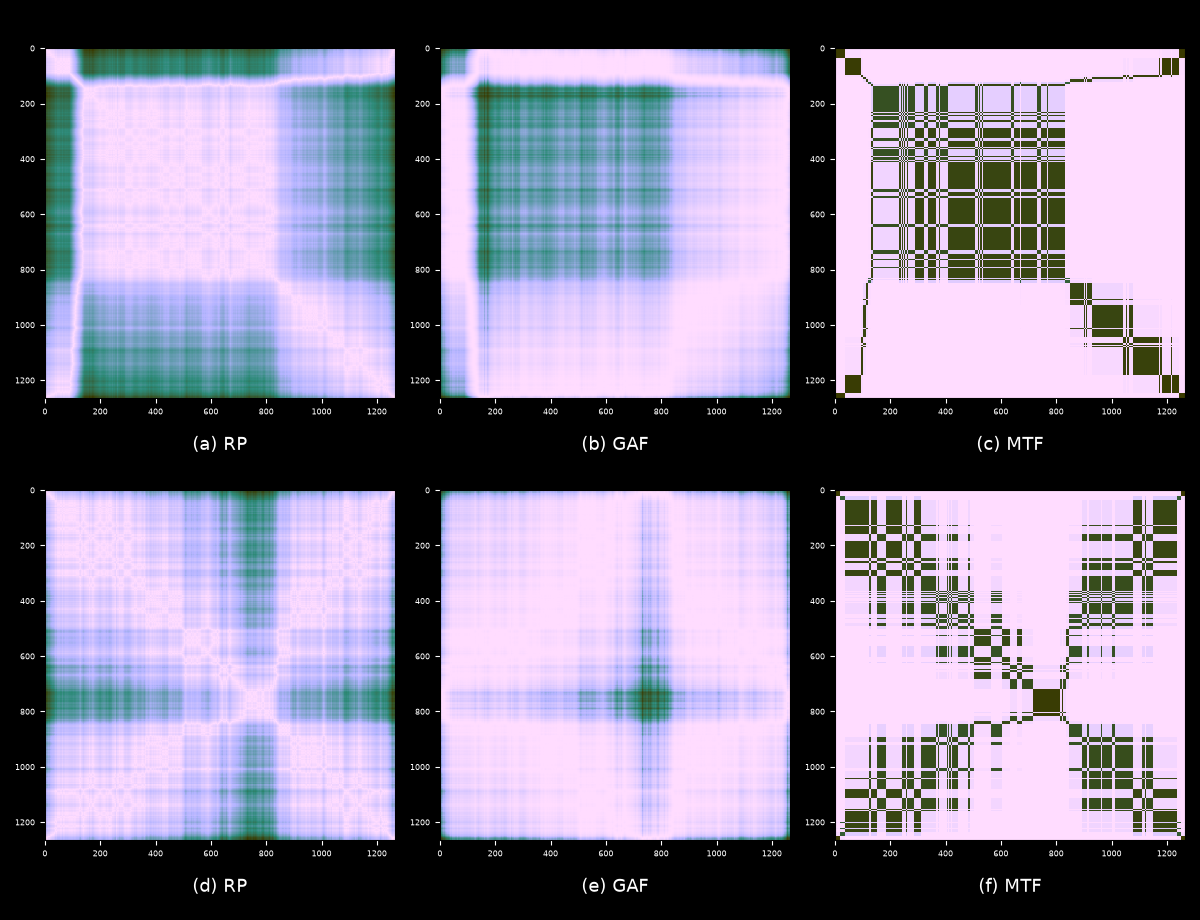
\includegraphics[width=\dimexpr0.80\textwidth-2\fboxsep\relax]{figures/image_transformation.png}}
    \caption{Sequence-to-image transformations for AY.4 (top row, a--c) and B.1.526 (bottom row, d--f). Columns show RP (a, d), GAF (b, e), and MTF (c, f).}
    \label{fig:image-transformation}
\end{figure*}

\subsection{Controls and Classical Surrogates}
\label{sec:controls}

To isolate the quantum contribution, all controls share the representation $x$, router, projection, classifier type, and mixing grid; they differ only in the feature map applied to $z_g$ (Table~\ref{tab:pqk-controls}).
\begin{itemize}
    \item \textit{C0} is the linear reference alone ($s=0$).
    \item \textit{C1} applies the Gaussian kernel directly to $z_g$, testing whether a feature map helps at all.
    \item \textit{C2} is a random-Fourier-feature (RFF) surrogate~\cite{rahimi2007rff,schreiber2023surrogates,sweke2023rff},
    \begin{equation}
        \phi^{\mathrm{RFF}}(z)=\big[\cos(\Omega^{\top}z+\beta),\ \sin(\Omega^{\top}z+\beta)\big]_{1:3n},
    \end{equation}
    with $\Omega_{ij}\sim\mathcal{N}(0,(2\tau)^2)$ and $\beta_i\sim\mathcal{U}[0,2\pi)$. Its scale matches the field band limit $2\tau$, and its output dimension and range match $\phi$. Because band-limited quantum models admit such surrogates~\cite{schreiber2023surrogates}, parity with C2 means that the quantum map is classically replaceable on this task.
    \item \textit{C3} removes all couplings. By Proposition~2, its kernel has the closed form
    \begin{equation}
        \kappa_{\mathrm{C3}}(z,z')=\prod_{k=1}^{n}\exp\!\big(-4\gamma\sin^2\!\big(\tau(z_k-z_k')\big)\big),
        \label{eq:c3-kernel}
    \end{equation}
    a classical, stationary, periodic kernel. MAIN$-$C3 is the comparison closest to isolating entanglement, but it is confounded: C3 also discards the coupling inputs (two LDA coordinates in D, one in B). A positive gap would therefore not identify entanglement as its cause. A null gap is still informative: the entangled map gains nothing even though it sees more inputs.
    \item \textit{C4} is a width-matched MLP (one $\tanh$ hidden layer of width $3n_g$) on $z_g$, with centered log-probabilities as scores.
    \item \textit{C5} uses a single PQK expert for all 22 lineages ($n=4$, $k=8$) without grouping.
\end{itemize}

\begin{table}[!t]
    \centering
    \caption{Configurations. All share $x$, the router, the projection, and the mixing grid.}
    \label{tab:pqk-controls}
    \footnotesize
    \setlength{\tabcolsep}{3pt}
    \renewcommand{\arraystretch}{1.15}
    \begin{tabularx}{\columnwidth}{@{}l>{\raggedright\arraybackslash}Xc>{\raggedright\arraybackslash}X@{}}
        \toprule
        ID & Feature map on $z_g$ & Grouped & Question addressed \\
        \midrule
        MAIN & PQK $\phi(z)$, entangled & \checkmark & --- \\
        C0 & none (reference only) & --- & Is the framework useful? \\
        C1 & identity, Gaussian kernel & \checkmark & Is any feature map useful? \\
        C2 & RFF surrogate, $3n$ dims & \checkmark & Is PQK classically replaceable? \\
        C3 & PQK without couplings & \checkmark & Is entanglement useful? \\
        C4 & MLP, width $3n$ & \checkmark & Equal-capacity network \\
        C5 & PQK, all 22 classes & --- & Is grouping useful? \\
        \bottomrule
    \end{tabularx}
\end{table}

\subsection{Decision Criteria Fixed in Advance}
\label{sec:criteria}

% TODO: cite the timestamped registry entry (Doc/registry/) to support
% "fixed before evaluation"; otherwise avoid the term "pre-registered".
For configurations $A$ and $B$ with mean test macro-F1 $F_A$, $F_B$ and seed standard deviations $\sigma_A$, $\sigma_B$, let $\Delta_{AB}=F_A-F_B$ and $\delta=0.02$, a noise floor estimated from repeated GPU runs in earlier experiments. A claim \emph{holds} if $\Delta_{AB}>\delta$ and $\Delta_{AB}>\max(\sigma_A,\sigma_B)$, is \emph{within noise} if $|\Delta_{AB}|\le\max(\delta,\sigma_A,\sigma_B)$, and \emph{fails} otherwise. The four claims are: the framework is useful (MAIN vs.\ C0); the quantum features are useful (MAIN vs.\ $\max\{\mathrm{C1},\mathrm{C2},\mathrm{C4}\}$, the strongest classical alternative); entanglement is useful (MAIN vs.\ C3); and grouping is useful (MAIN vs.\ C5). If neither quantum claim holds, PQK is declared classically replaceable on this task, and enlarging $n$ or retuning $(T,\tau,\gamma)$ to reverse the outcome is not permitted. With the single seed reported here, $\sigma_A=\sigma_B=0$ and the criteria reduce to the fixed floor $\delta$.

% =====================================================================
\section{Results}
\label{sec:result}
% Baseline results are transcribed from references/classical_overview.md and
% references/cnn_overview.md. QuSpike-PQK results are from
% Results/quspike_pqk/pqk_{MAIN,C0..C5}__mut__seed0.json.

We answer the research question in three steps: how QuSpike-PQK compares with existing baselines (Section~\ref{sec:res-baselines}), whether that result is due to the quantum component (Section~\ref{sec:res-controls}), and what the kernels and costs reveal about why (Sections~\ref{sec:res-kernel} and~\ref{sec:res-cost}).

\subsection{Comparison with Baselines}
\label{sec:res-baselines}

Table~\ref{tab:classification-results} and Fig.~\ref{fig:compare} compare the classical, image-CNN, and QuSpike-PQK results on the 22-class task.

\textbf{Embedding-based baselines.} One-hot LR achieves the highest macro-F1 (0.7339), while RF performs best on autoencoder embeddings (0.5696); all seven classifiers obtain higher macro-F1 with one-hot inputs than with autoencoder embeddings. However, one-hot LR reached the iteration limit without convergence, and MLP also produced convergence warnings.

\textbf{Image-based baselines.} All nine CNN configurations use seed 0 only. The best is the four-layer CNN with RP (macro-F1 0.6787, accuracy 0.6333), almost level with GAF (0.6755); MTF is clearly worse (0.465--0.569). Deeper networks help (the four-layer CNN is about 0.04--0.08 above the three-layer one), but ResNet34 is not better (0.6633 with RP), and its training loss is far below that of the four-layer CNN, indicating overfitting. The best image-CNN macro-F1 is below the best one-hot classical method (0.7339), yet its training time is one to two orders of magnitude higher (80--156 minutes). Ancestral and Delta sublineages such as AY.103, B.1, B.1.1, B.1.617.2, AY.3, and AY.44 are the hardest to separate for every CNN.

\textbf{QuSpike-PQK.} QuSpike-PQK reaches a macro-F1 of 0.7547, $+0.021$ above the best classical baseline (one-hot LR, 0.7339) and $+0.076$ above the best image CNN (four-layer CNN with RP, 0.6787). Its accuracy is 0.6893 (best classical 0.6783, best CNN 0.6333), macro precision 0.7692, macro recall 0.7594, and ROC AUC 0.9745, the highest values in the table. Training takes 3.09 minutes, about 29 times less than the best CNN, 49 times less than ResNet34, and less than the 6.17 minutes of one-hot LR. The margin over one-hot LR is only just above the noise floor $\delta$ and is measured on slightly different sample sets (Section~\ref{sec:baselines}), so it should not be over-interpreted. More importantly, the next subsection shows that it is not a quantum effect: the linear reference C0 alone already reaches 0.7481, so most of the margin over one-hot LR comes from the mutation-indicator representation.

For QuSpike-PQK and most of the stronger baselines, macro-F1 exceeds accuracy. Accuracy is dominated by the four largest lineages (900 test sequences each), three of which are hard (QuSpike-PQK F1: AY.103 0.474, AY.44 0.492, B.1.2 0.667), whereas macro-F1 weights small, well-separated lineages equally (e.g., AY.2 0.966 on 14 test sequences).

\begin{figure}[!t]
    \centering
    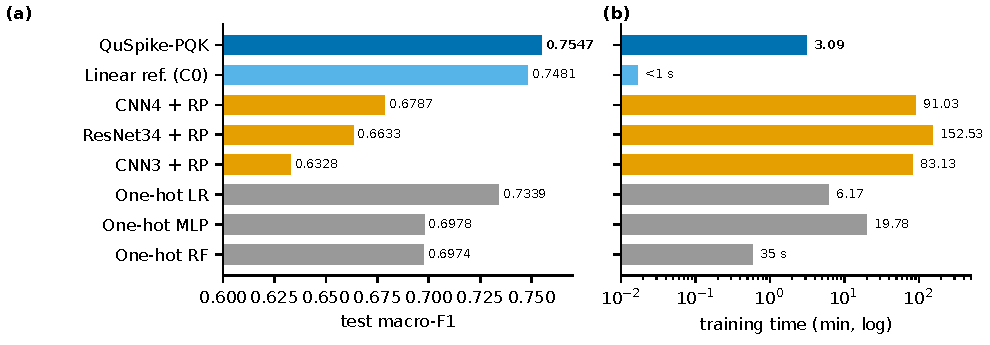
\includegraphics[width=\columnwidth]{figures/fig_compare.pdf}
    \caption{QuSpike-PQK versus representative baselines (22-class task). (a) Test macro-F1; (b) training time (log scale, minutes). Gray: one-hot classical classifiers; orange: image CNNs (RP of each); light blue: our linear reference (C0); dark blue: QuSpike-PQK. All results are from a single seed.}
    \label{fig:compare}
\end{figure}

\begin{table*}[!t]
    \centering
    \caption{Baseline and QuSpike-PQK results on the 22-class task. Bold values mark the best scores within each family; the QuSpike-PQK row is shaded.}
    \label{tab:classification-results}
    \footnotesize
    \setlength{\tabcolsep}{2.7pt}
    \renewcommand{\arraystretch}{1.2}
    \newcommand{\resultpending}{\textemdash}
    \begin{tabular*}{\textwidth}{@{\extracolsep{\fill}}>{\raggedright\arraybackslash}p{0.11\textwidth}>{\raggedright\arraybackslash}p{0.14\textwidth}lrrrrrrr@{}}
        \toprule
        Approach & Embedding & Algorithm & Acc. & \shortstack{Prec.\\(Macro)} & \shortstack{Recall\\(Macro)} &
        \shortstack{F1\\(Weighted)} & \shortstack{F1\\(Macro)} &
        \shortstack{ROC AUC\\(OvR)} & Train time \\
        \midrule
        \multirow{14}{=}{Embedding-based (22 classes)} & \multirow{7}{=}{One-hot} & SVM & 0.5542 & 0.4768 & 0.4642 & 0.4904 & 0.4410 & 0.9382 & 6.32~m \\
         &  & NB & 0.3626 & 0.3274 & 0.3287 & 0.3090 & 0.2622 & 0.8596 & \(<1.00\)~s \\
         &  & MLP & \(0.6523 \pm 0.0094\) & 0.7239 & 0.7068 & 0.6438 & \(0.6978 \pm 0.0190\) & 0.9626 & 19.78~m \\
         &  & KNN & 0.6021 & 0.6754 & 0.6282 & 0.5916 & 0.6409 & 0.8830 & \(<1.00\)~s \\
         &  & RF & \(0.6593 \pm 0.0013\) & 0.7217 & 0.7006 & 0.6450 & \(0.6974 \pm 0.0019\) & 0.9559 & 35.00~s \\
         &  & LR\textsuperscript{*} & \(\mathbf{0.6783} \pm 0.0000\) & \textbf{0.7379} & \textbf{0.7443} & \textbf{0.6707} & \(\mathbf{0.7339} \pm 0.0000\) & \textbf{0.9671} & 6.17~m \\
         &  & DT & \(0.6424 \pm 0.0020\) & 0.6873 & 0.7179 & 0.6351 & \(0.6927 \pm 0.0065\) & 0.8534 & 24.00~s \\
        \cmidrule(l){2-10}
         & \multirow{7}{=}{Autoencoder (128-D)} & SVM & \(0.4933 \pm 0.0099\) & 0.4220 & 0.4110 & 0.4166 & \(0.3792 \pm 0.0228\) & 0.8979 & \resultpending \\
         &  & NB & \(0.2134 \pm 0.0222\) & 0.3314 & 0.3092 & 0.2242 & \(0.2418 \pm 0.0191\) & 0.7949 & \resultpending \\
         &  & MLP & \(0.5477 \pm 0.0118\) & 0.5235 & 0.5518 & 0.5213 & \(0.5185 \pm 0.0175\) & 0.9246 & \resultpending \\
         &  & KNN & \(0.5451 \pm 0.0074\) & 0.5656 & 0.5620 & 0.5352 & \(0.5516 \pm 0.0131\) & 0.8562 & \resultpending \\
         &  & RF & \(0.5769 \pm 0.0071\) & 0.6092 & 0.5784 & 0.5639 & \(0.5696 \pm 0.0125\) & 0.9233 & \resultpending \\
         &  & LR & \(0.5353 \pm 0.0150\) & 0.5021 & 0.5117 & 0.4842 & \(0.4842 \pm 0.0223\) & 0.9217 & \resultpending \\
         &  & DT & \(0.5166 \pm 0.0038\) & 0.5028 & 0.5318 & 0.5124 & \(0.5130 \pm 0.0090\) & 0.7541 & \resultpending \\
        \midrule
        \multirow{9}{=}{Image-based (22 classes)} & RP & \multirow{3}{*}{3-layer CNN} & 0.6149 & 0.6890 & 0.6539 & 0.5700 & 0.6328 & 0.9637 & 83.13~m \\
         & GAF &  & 0.6092 & 0.6754 & 0.6432 & 0.5614 & 0.6197 & 0.9624 & 85.85~m \\
         & MTF &  & 0.5179 & 0.5410 & 0.4781 & 0.4640 & 0.4649 & 0.9350 & 80.53~m \\
        \cmidrule(l){2-10}
         & RP & \multirow{3}{*}{4-layer CNN} & \textbf{0.6333} & \textbf{0.6920} & 0.6868 & \textbf{0.6185} & \textbf{0.6787} & \textbf{0.9640} & 91.03~m \\
         & GAF &  & 0.6256 & 0.6886 & \textbf{0.6887} & 0.6096 & 0.6755 & 0.9616 & 93.75~m \\
         & MTF &  & 0.5316 & 0.5901 & 0.5391 & 0.5155 & 0.5464 & 0.9343 & 88.43~m \\
        \cmidrule(l){2-10}
         & RP & \multirow{3}{*}{ResNet34} & 0.6163 & 0.6610 & 0.6848 & 0.6093 & 0.6633 & 0.9410 & 152.53~m \\
         & GAF &  & 0.6069 & 0.6453 & 0.6749 & 0.5993 & 0.6532 & 0.9437 & 155.53~m \\
         & MTF &  & 0.5544 & 0.5732 & 0.5819 & 0.5467 & 0.5693 & 0.9271 & 150.37~m \\
        \midrule
        \rowcolor{blue!10} \textbf{Proposed (22 classes)} & \textbf{Mutation indicator} & \textbf{QuSpike-PQK} & \textbf{0.6893} & \textbf{0.7692} & \textbf{0.7594} & \textbf{0.6863} & \textbf{0.7547} & \textbf{0.9745} & \textbf{3.09~m} \\
        \bottomrule
    \end{tabular*}
    \par\smallskip
    \begin{minipage}{\textwidth}
        \footnotesize
        Classical Acc. and macro-F1 show mean $\pm$ sample standard deviation when available; other classical metrics show means. Autoencoder runs use five seeds; one-hot SVM, NB, and KNN use one run, and the other one-hot models use five seeds. CNN scores are from seed 0 only (cumulative-sum signals; the 3-/4-layer CNNs and ResNet34 are trained for 100 epochs; ResNet34 is ImageNet-pretrained). QuSpike-PQK is from seed 0 only and uses 22,175 training and 9,514 test sequences; its training time covers the linear reference, mixing-weight search, quantum features, and kernel SVMs. $^{*}$One-hot LR did not converge. Autoencoder training times are omitted because they include representation training. Dashes indicate unreported values. RP: recurrence plot; GAF: Gramian angular field; MTF: Markov transition field. Metrics are on a 0--1 scale; training time uses seconds (s), minutes (m), or hours (h), with two decimal places.
    \end{minipage}
\end{table*}

\subsection{Matched Controls: Is the Gain Quantum?}
\label{sec:res-controls}

Table~\ref{tab:control-results} lists all configurations, and Table~\ref{tab:claims} evaluates the four claims of Section~\ref{sec:criteria}. All configurations share a routing accuracy of $\rho=0.9667$.

\begin{table}[!t]
    \centering
    \caption{Matched controls (seed 0, test set). $s^\star$: validation-selected mixing weight; $F_{\mathrm{D}}$, $F_{\mathrm{B}}$: group macro-F1 (Section~\ref{sec:metrics}); group O stays at 0.949 in every configuration.}
    \label{tab:control-results}
    \footnotesize
    \setlength{\tabcolsep}{4pt}
    \renewcommand{\arraystretch}{1.12}
    \begin{tabular*}{\columnwidth}{@{\extracolsep{\fill}}lccccc@{}}
        \toprule
        Config & Macro-F1 & Acc. & $F_{\mathrm{D}}$ & $F_{\mathrm{B}}$ & $s^\star$ \\
        \midrule
        \rowcolor{blue!10} MAIN (PQK) & 0.7547 & 0.6893 & 0.612 & 0.567 & 0.25 \\
        C0 (reference) & 0.7481 & 0.6847 & 0.601 & 0.550 & 0 \\
        C1 (Gaussian on $z$) & 0.7534 & 0.6877 & 0.609 & 0.565 & 0.5 \\
        C2 (RFF surrogate) & \textbf{0.7552} & \textbf{0.6898} & 0.612 & \textbf{0.570} & 0.25 \\
        C3 (no coupling) & 0.7544 & 0.6891 & \textbf{0.613} & 0.563 & 0.5 \\
        C4 (MLP) & 0.7489 & 0.6834 & 0.600 & 0.557 & 0.25 \\
        C5 (ungrouped) & 0.7481 & 0.6847 & 0.601 & 0.550 & 0 \\
        \bottomrule
    \end{tabular*}
\end{table}

\begin{table}[!t]
    \centering
    \caption{Decisions on the claims fixed in advance ($\delta=0.02$, single seed). $^{\dagger}$C2 is the strongest of C1, C2, and C4.}
    \label{tab:claims}
    \footnotesize
    \setlength{\tabcolsep}{3pt}
    \renewcommand{\arraystretch}{1.12}
    \begin{tabular*}{\columnwidth}{@{\extracolsep{\fill}}llrl@{}}
        \toprule
        Claim & Comparison & $\Delta$ & Decision \\
        \midrule
        Framework useful & MAIN $-$ C0 & $+0.0066$ & within noise \\
        Quantum features useful & MAIN $-$ C2$^{\dagger}$ & $-0.0005$ & within noise \\
        Entanglement useful & MAIN $-$ C3 & $+0.0003$ & within noise \\
        Grouping useful & MAIN $-$ C5 & $+0.0066$ & within noise \\
        \bottomrule
    \end{tabular*}
\end{table}

Relative to its own linear reference, MAIN gains $+0.0066$ macro-F1. By Proposition~3, this gain comes entirely from the two expert groups: group macro-F1 rises from 0.601 to 0.612 for Delta and from 0.550 to 0.567 for the B.1 family, while group O stays at 0.949. Every matched classical control does as well. The RFF surrogate C2 (0.7552) and the entanglement-free circuit C3 (0.7544) are level with MAIN, the Gaussian kernel on $z$ (C1, 0.7534) is close behind, and the width-matched MLP (C4, 0.7489) recovers part of the gain. The ungrouped expert C5 selects $s=0$ on validation and therefore coincides with C0 (Fig.~\ref{fig:results-viz}a).

All four claims are within noise (Table~\ref{tab:claims}), which triggers the stopping rule: \emph{on this task, the projected quantum kernel is classically replaceable}. The small gain over C0 is shared by every feature map applied to the group-wise LDA coordinates, so it is better attributed to the residual group experts than to the quantum circuit.

\begin{figure}[!t]
    \centering
    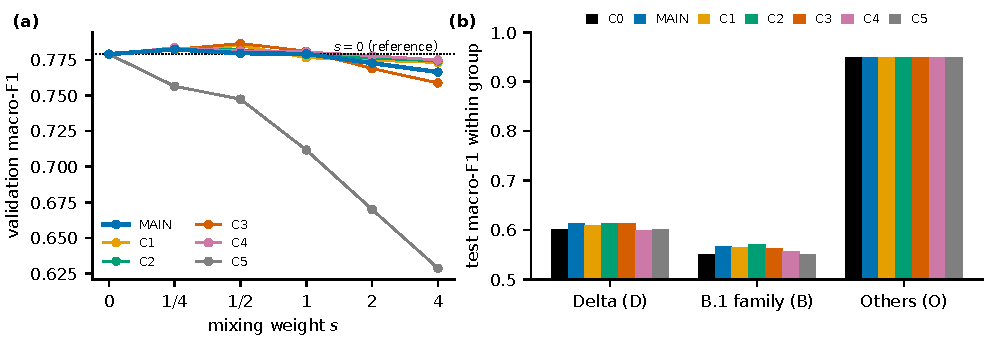
\includegraphics[width=\columnwidth]{figures/fig_results.pdf}
    \caption{QuSpike-PQK experimental results (seed 0). (a) Validation macro-F1 versus the mixing weight $s$: all configurations start from the same point at $s=0$ (reference only); MAIN peaks at $s=0.25$, while C5 (ungrouped) drops quickly as $s$ grows and therefore selects $s=0$, equal to C0. (b) Test group macro-F1: all gains come from groups D and B, and group O stays at 0.949 in every configuration.}
    \label{fig:results-viz}
\end{figure}

\subsection{Kernel Structure}
\label{sec:res-kernel}

Figure~\ref{fig:gram} compares the Gram matrices of MAIN with the classical RBF kernel on $z$ (C1). In all three groups, the gap between mean same-lineage and cross-lineage kernel values is no larger for MAIN (D 0.222, B 0.176, O 0.725) than for the classical RBF (0.244, 0.249, 0.733), so the quantum kernel shows no better class structure.

The difficult lineages are difficult under both kernels. In group D, AY.25 and AY.4 form their own blocks, but kernel values among AY.103, AY.3, and AY.44 are high (about 0.6--0.8). In group B, with only 2 qubits and a 3-dimensional LDA, the cross-lineage kernel value of MAIN is as high as 0.404 and only B.1.177 is clearly separated. In group O, both kernels give nearly block-diagonal matrices, with a clear high-similarity block only between B.1.427 and B.1.429. The same lineages overlap already in the LDA projection (Fig.~\ref{fig:lda-scatter}), before any feature map is applied.

\begin{figure*}[!t]
    \centering
    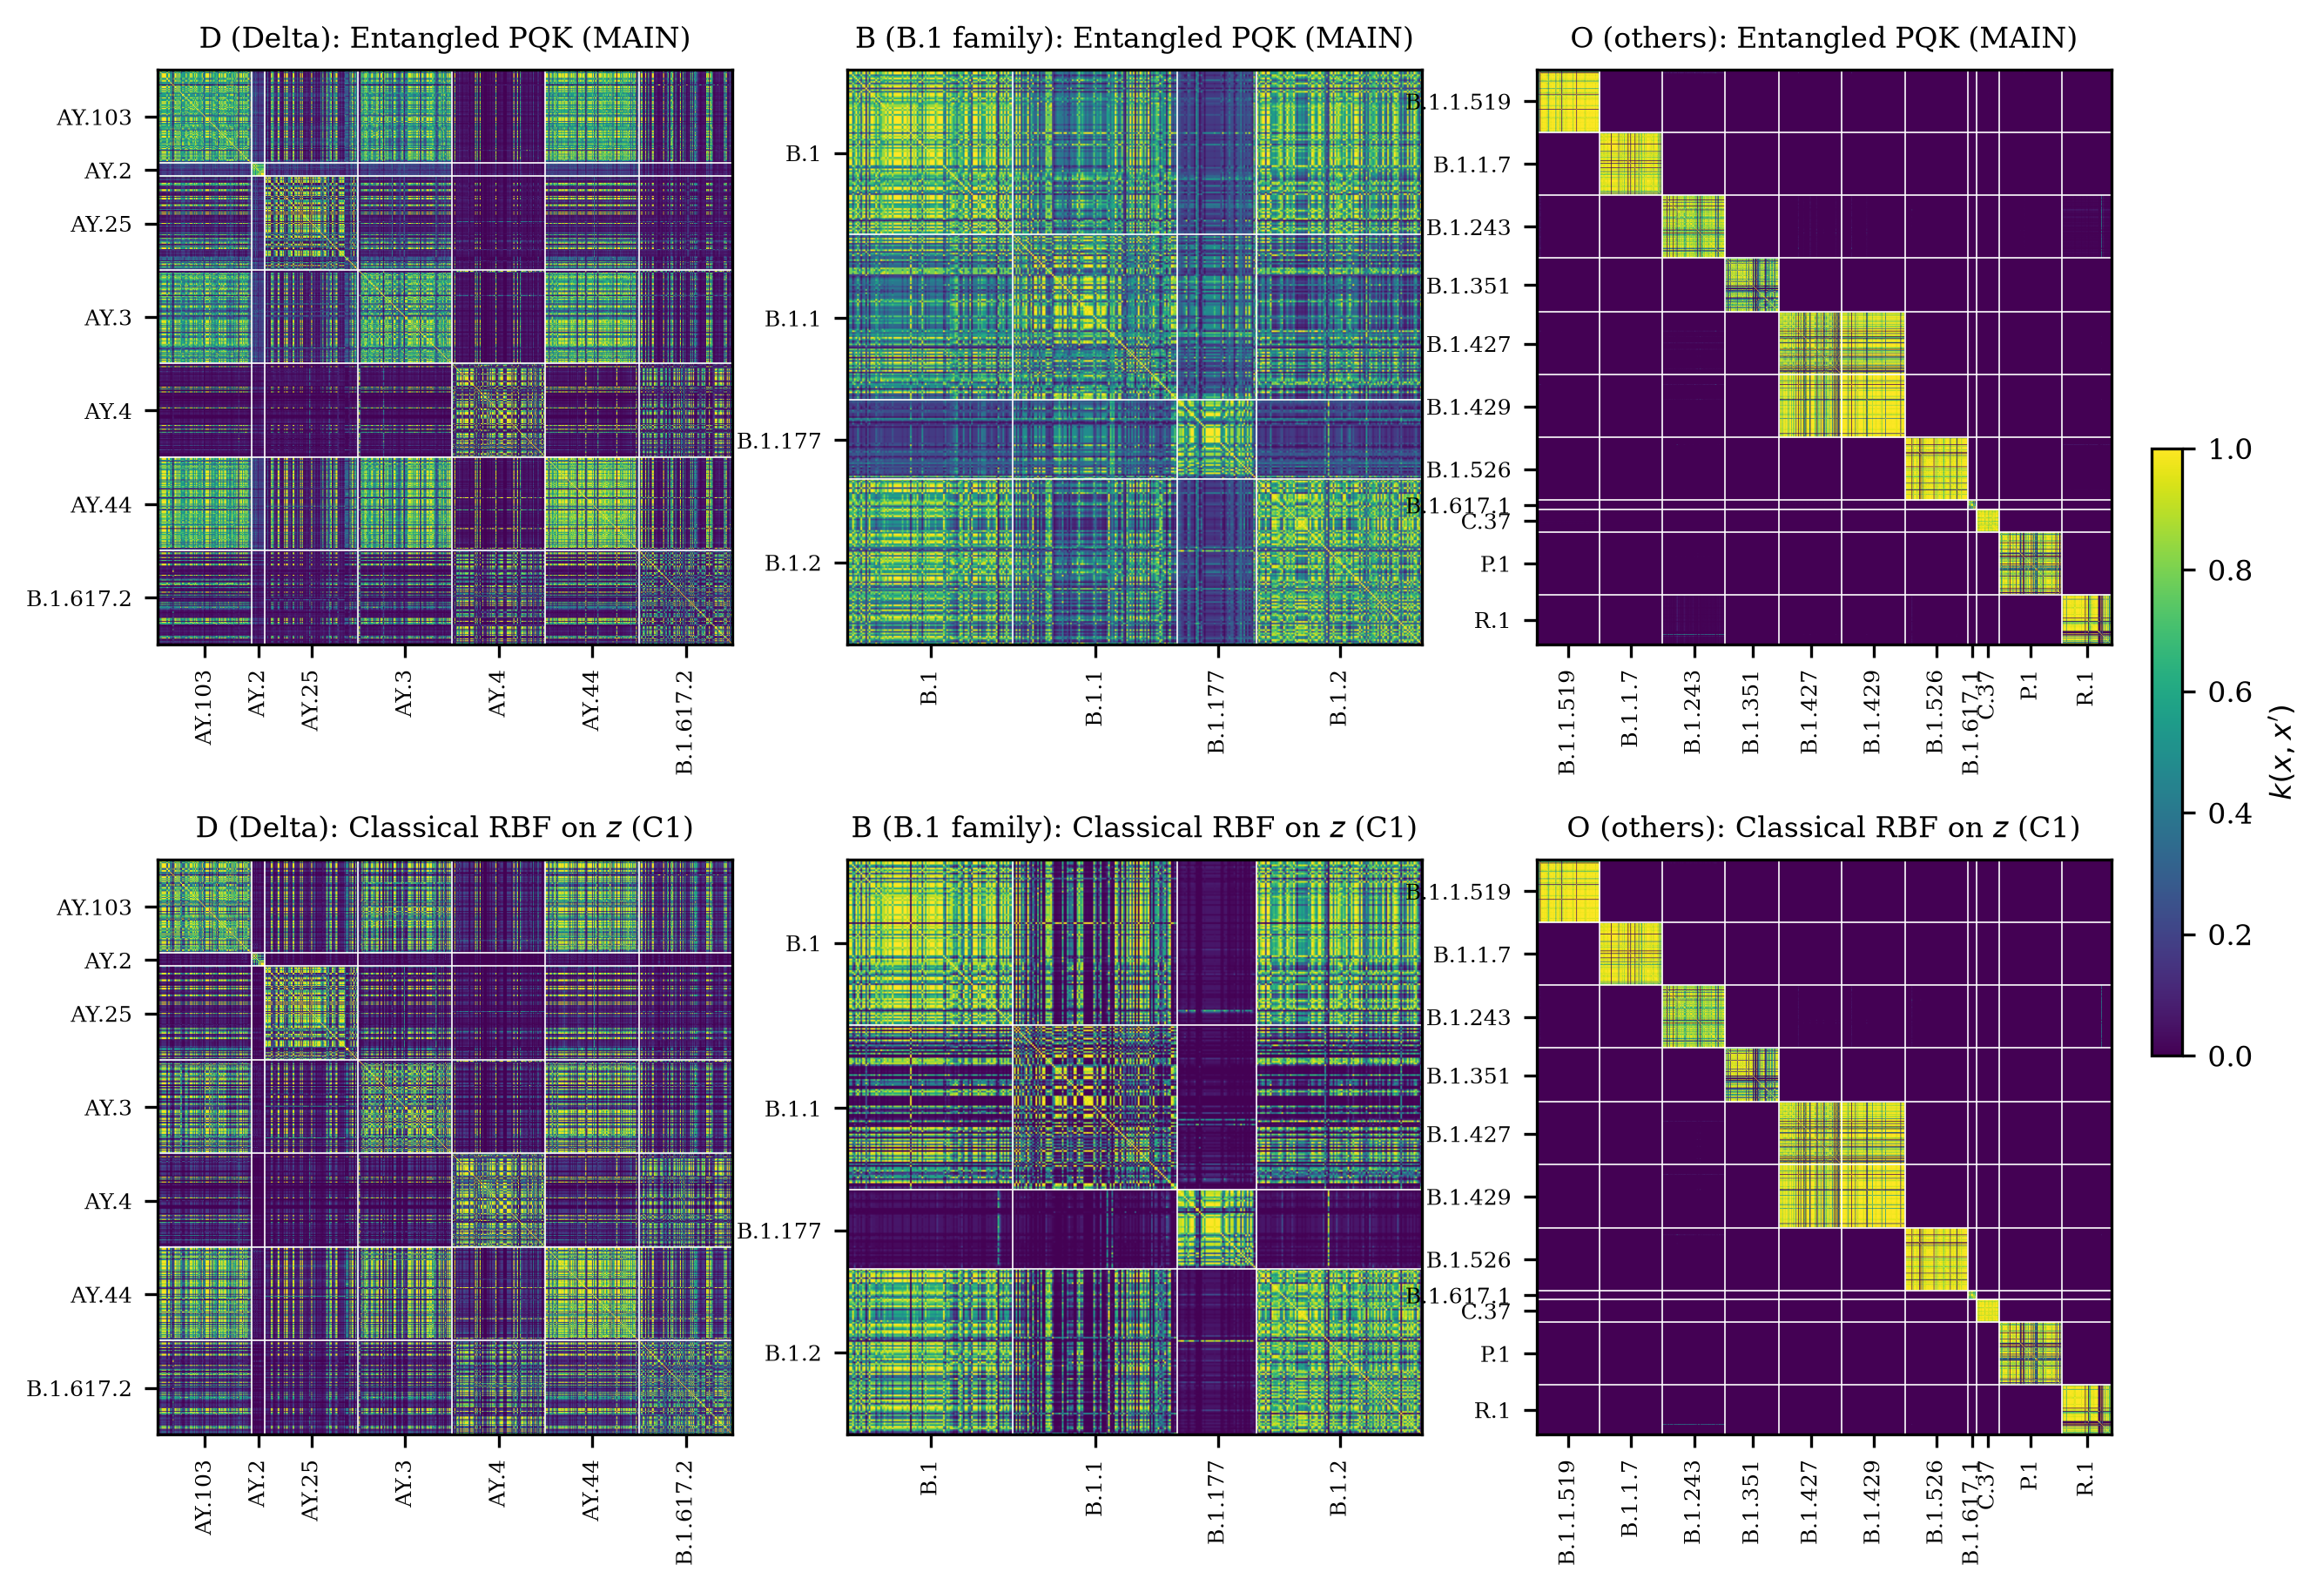
\includegraphics[width=0.92\textwidth]{figures/gram_groups.png}
    \caption{Gram matrices of the three groups (sorted by lineage, white lines mark lineage boundaries; the first 100 test sequences per lineage, or all if fewer). Top row: entangled PQK (MAIN); bottom row: classical RBF computed directly on $z$ (C1). Columns: D (Delta, 4 qubits), B (B.1 family, 2 qubits), and O (others; computed with $n=4$ here for comparison only). Mean same-/cross-lineage kernel values (MAIN) are D 0.467/0.245, B 0.580/0.404, and O 0.745/0.020; the gaps (MAIN versus C1) are D 0.222 vs 0.244, B 0.176 vs 0.249, and O 0.725 vs 0.733.}
    \label{fig:gram}
\end{figure*}

\subsection{Runtime}
\label{sec:res-cost}

MAIN runs for 185~s end to end, of which the quantum features for the 19,630 training and test sequences of groups D and B take 0.37~s; the rest is spent mainly in the kernel SVMs. Across the kernel-based configurations (MAIN, C1, C2, C3, C5), the end-to-end time ranges from 138 to 576~s. As predicted in Section~\ref{sec:complexity}, the classical kernel machine, not the quantum feature map, is the bottleneck.

% =====================================================================
\section{Discussion}
\label{sec:discussion}

\subsection{Why the Quantum Features Do Not Help}
\label{sec:why}

Three observations point to the same explanation: the remaining errors come from information the expert never receives, not from the expressiveness of the feature map.

\textit{Information bottleneck.} The circuit sees only $k_g\le2n_g$ LDA coordinates of a $V=3{,}686$-dimensional input. By the data-processing inequality, $I(y;\phi(z_g))\le I(y;z_g)\le I(y;x)$, so no feature map can recover discriminative information discarded by the projection. Proposition~1 further reduces the readout to $3n-1$ effective dimensions, and zero padding decouples one qubit in group D. The lineages that remain confused (AY.103, AY.3, AY.44; B.1, B.1.1, B.1.2) already overlap in the LDA projection (Fig.~\ref{fig:lda-scatter}).

\textit{Spike-only information.} The same inequality applies one level earlier, to $I(y;x)\le I(y;\text{genome})$. Pango lineages are assigned from whole-genome mutation patterns~\cite{rambaut2020pango,otoole2021pangolin}, and several sublineage distinctions within groups D and B are carried largely by mutations outside the spike gene.
% TODO: verify with lineage-defining mutations (e.g., cov-lineages.org):
% AY.x sublineages vs. B.1.617.2, and B.1 vs. B.1.1 (N:R203K/G204R).
If so, the confusion within D and B reflects a ceiling of the spike-only representation that no classifier on $x$ can lift, which is consistent with every configuration in Table~\ref{tab:control-results} plateauing at nearly the same group scores.

\textit{Band-limited, low-dimensional map.} With $n\le4$ and $T=4$, the readout is a low-degree trigonometric polynomial of $z$ (Section~\ref{sec:encoding}) that RFF approximates closely (Fig.~\ref{fig:viz-encoding}b); C2 is therefore expected to match MAIN, and it does.

\subsection{Limitations}
\label{sec:limitations}

(L1) \emph{Classical simulability.} At $n\le4$, the model is simulated exactly at negligible cost. Scaling $n$ at fixed $T$ does not by itself make it hard to simulate: single-qubit marginals of shallow nearest-neighbor circuits can be computed from their backward light cones in time exponential only in the depth. (L2) \emph{Dequantization.} The band-limited spectrum admits RFF surrogates~\cite{schreiber2023surrogates,sweke2023rff}, which C2 instantiates. (L3) \emph{Confounded entanglement control.} C3 removes the coupling inputs together with the entanglement; a cleaner control would feed the coupling coordinates to additional product-state fields. (L4) \emph{Concentration at scale.} For larger, more entangling evolutions, 1-RDMs approach the maximally mixed state, $\phi\to0$, and kernel values concentrate~\cite{thanasilp2024concentration}; the median-heuristic $\gamma$ then grows and amplifies the shot-noise bound of Section~\ref{sec:noise}. (L5) \emph{Hardware cost.} Each sequence needs three settings of $S$ shots. A dry-run estimate for the Delta test set alone is about 3.5~h of device time in 164 jobs, and the classical $O(N_g^2)$ kernel machine remains. (L6) \emph{Statistical evidence.} All QuSpike-PQK results come from a single seed, and the noise floor $\delta$ was estimated in earlier experiments rather than for this model; multiple seeds and paired tests on the test set are needed to confirm the decisions. (L7) \emph{Positioning.} The framework claims no quantum advantage or speedup. Its purpose is to make parity or gain decidable on a real task with strong classical baselines, in line with recent benchmarking guidance~\cite{bowles2024better}.

\subsection{When Could a PQK Help?}
\label{sec:when}

Proposition~5(iii) gives only a necessary condition against exact simulation ($n\gtrsim\log_2 3S$). Quantum advantage would additionally require: (a) a feature map that cannot be dequantized, i.e., lies outside the band-limited regime that RFF can approximate~\cite{schreiber2023surrogates,sweke2023rff}, and whose single-qubit marginals cannot be computed efficiently from shallow light cones (L1); (b) kernel values that do not concentrate exponentially in $n$~\cite{thanasilp2024concentration}, since otherwise $\gamma$, and with it the required $S$, grows (Section~\ref{sec:noise}); and (c) discriminative information that genuinely resides in the quantum features, i.e., outperforming classical surrogates, which, as shown by Huang \textit{et al.}~\cite{huang2021power}, requires data-dependent quantum structure. The C2 and C3 controls show that (a) and (c) are not met for $n\le4$ on this dataset. A task in which these conditions might hold would also need an input that the classical projection does not already reduce to a few separable coordinates.

% =====================================================================
\section{Conclusion}
\label{sec:conclusion}

We asked whether a fixed quantum feature map adds discriminative information beyond matched classical alternatives on SARS-CoV-2 spike-lineage classification. QuSpike-PQK, which adds group-wise projected-quantum-kernel experts to a linear reference on mutation indicators, reaches a macro-F1 of 0.7547 on 22 lineages, above one-hot and image-CNN baselines and at a fraction of the training time. The matched controls show that this result does not depend on the quantum component: a random-Fourier-feature surrogate, an entanglement-free circuit, and a Gaussian kernel on the same coordinates perform equally well, and most of the margin over the baselines comes from the mutation-indicator representation. On this task the projected quantum kernel is therefore classically replaceable. The architecture and control protocol remain useful as a template: they make a quantum contribution attributable, keep the quantum workload linear in the data, and turn a claim of quantum benefit into a decision that can fail. Future work should run multiple seeds with label-free inference, add an input-matched entanglement control, measure the spike-only information ceiling, and test the protocol on tasks where the conditions of Section~\ref{sec:when} are plausible.

% Keep every results float ahead of the References section.
\FloatBarrier
\begin{thebibliography}{00}
\bibitem{murad2024snn}
T.~Murad, P.~Chourasia, S.~Ali, I.~U.~Khan, and M.~Patterson,
``Neuromorphic spiking neural network based classification of COVID-19 spike sequences,''
arXiv:2501.14746, 2024.

\bibitem{ncbiSarsStructure}
National Center for Biotechnology Information,
``SARS-CoV-2 conserved domains and 3D structures.''
[Online]. Available: \url{https://www.ncbi.nlm.nih.gov/Structure/SARS-CoV-2.html}

% TODO: verify the four lineage-assignment entries below against the publishers.
\bibitem{rambaut2020pango}
A.~Rambaut \textit{et al.},
``A dynamic nomenclature proposal for SARS-CoV-2 lineages to assist genomic epidemiology,''
\textit{Nature Microbiology}, vol.~5, pp.~1403--1407, 2020.

\bibitem{otoole2021pangolin}
\'{A}.~O'Toole \textit{et al.},
``Assignment of epidemiological lineages in an emerging pandemic using the pangolin tool,''
\textit{Virus Evolution}, vol.~7, no.~2, Art.~veab064, 2021.

\bibitem{turakhia2021usher}
Y.~Turakhia \textit{et al.},
``Ultrafast Sample placement on Existing tRees (UShER) enables real-time phylogenetics for the SARS-CoV-2 pandemic,''
\textit{Nature Genetics}, vol.~53, pp.~809--816, 2021.

\bibitem{aksamentov2021nextclade}
I.~Aksamentov, C.~Roemer, E.~B.~Hodcroft, and R.~A.~Neher,
``Nextclade: Clade assignment, mutation calling and quality control for viral genomes,''
\textit{Journal of Open Source Software}, vol.~6, no.~67, Art.~3773, 2021.

\bibitem{maass1997}
W.~Maass,
``Networks of spiking neurons: The third generation of neural network models,''
\textit{Neural Networks}, vol.~10, no.~9, pp.~1659--1671, 1997.

\bibitem{pfeiffer2018}
M.~Pfeiffer and T.~Pfeil,
``Deep learning with spiking neurons: Opportunities and challenges,''
\textit{Frontiers in Neuroscience}, vol.~12, Art.~774, 2018.

\bibitem{cerezo2021vqa}
M.~Cerezo \textit{et al.},
``Variational quantum algorithms,''
\textit{Nature Reviews Physics}, vol.~3, pp.~625--644, 2021,
doi: 10.1038/s42254-021-00348-9.
% Verified source: https://arxiv.org/abs/2012.09265
\bibitem{huang2021power}
H.-Y.~Huang, M.~Broughton, M.~Mohseni, R.~Babbush, S.~Boixo, H.~Neven, and J.~R.~McClean,
``Power of data in quantum machine learning,''
\textit{Nature Communications}, vol.~12, Art.~2631, 2021.
% arXiv:2011.01938

\bibitem{schuld2021effect}
M.~Schuld, R.~Sweke, and J.~J.~Meyer,
``Effect of data encoding on the expressive power of variational quantum-machine-learning models,''
\textit{Physical Review A}, vol.~103, Art.~032430, 2021.
% arXiv:2008.08605

\bibitem{schreiber2023surrogates}
F.~J.~Schreiber, J.~Eisert, and J.~J.~Meyer,
``Classical surrogates for quantum learning models,''
\textit{Physical Review Letters}, vol.~131, Art.~100803, 2023.
% arXiv:2206.11740

\bibitem{sweke2023rff}
R.~Sweke, E.~Recio-Armengol, S.~Jerbi, E.~Gil-Fuster, B.~Fuller, J.~Eisert, and J.~J.~Meyer,
``Potential and limitations of random Fourier features for dequantizing quantum machine learning,''
arXiv:2309.11647, 2023.

\bibitem{rahimi2007rff}
A.~Rahimi and B.~Recht,
``Random features for large-scale kernel machines,''
in \textit{Advances in Neural Information Processing Systems}, vol.~20, 2007.

\bibitem{havlicek2019}
V.~Havl\'{i}\v{c}ek \textit{et al.},
``Supervised learning with quantum-enhanced feature spaces,''
\textit{Nature}, vol.~567, pp.~209--212, 2019.

\bibitem{lloyd1996}
S.~Lloyd,
``Universal quantum simulators,''
\textit{Science}, vol.~273, no.~5278, pp.~1073--1078, 1996.

\bibitem{childs2021trotter}
A.~M.~Childs, Y.~Su, M.~C.~Tran, N.~Wiebe, and S.~Zhu,
``Theory of Trotter error with commutator scaling,''
\textit{Physical Review X}, vol.~11, Art.~011020, 2021.

\bibitem{fisher1936}
R.~A.~Fisher,
``The use of multiple measurements in taxonomic problems,''
\textit{Annals of Eugenics}, vol.~7, no.~2, pp.~179--188, 1936.

\bibitem{williams2001nystrom}
C.~K.~I.~Williams and M.~Seeger,
``Using the Nystr\"om method to speed up kernel machines,''
in \textit{Advances in Neural Information Processing Systems}, vol.~13, 2001.

\bibitem{mcclean2018barren}
J.~R.~McClean, S.~Boixo, V.~N.~Smelyanskiy, R.~Babbush, and H.~Neven,
``Barren plateaus in quantum neural network training landscapes,''
\textit{Nature Communications}, vol.~9, Art.~4812, 2018.

\bibitem{thanasilp2024concentration}
S.~Thanasilp, S.~Wang, M.~Cerezo, and Z.~Holmes,
``Exponential concentration in quantum kernel methods,''
\textit{Nature Communications}, vol.~15, Art.~5200, 2024.
% arXiv:2208.11060

\bibitem{bowles2024better}
J.~Bowles, S.~Ahmed, and M.~Schuld,
``Better than classical? The subtle art of benchmarking quantum machine learning models,''
arXiv:2403.07059, 2024.
% TODO: verify volume/article numbers of the entries above against the publishers.
\end{thebibliography}

\end{document}
